
En este caso, se generaron arreglos con datos aleatorios de tamaños $10^{1} , 10^{3}$ y $10^{5}$, donde el dominio de los datos puede ser: ${D1,D7}$, donde D1 quiere decir que cada valor del arreglo es un entero entre 0 y 9, para D7 cada valor va entre 0 y $10^{7}$. Para las matrices se generaron aleatoriamente con tamaños $2^{4}$ , $2^{6}$ y $2^{8} $, donde el dominio de los datos puede ser: ${D0,D10}$, donde en D0 los valores son binarios : {0,1} y en D10 son enteros entre 0 y 9. El tiempo se
midió con std::chrono::high\_resolution\_clock y la memoria mediante el incremento del pico de memoria residente (VmHWM en /proc/self/status) antes y después de cada ejecución.



\subsection{Ordenamiento de arreglos unidimensionales}

Antes de comenzar el análisis, es importante conocer la complejidad temporal y espacial teórica de los algoritmos implementados. Además, cabe aclarar que se cambió la implementación de $QuickSort$, haciendo que el pivote fuera elegido aleatoriamente.

\begin{table}[!h]
\centering
\label{tab:complejidades_sort}
\begin{tabular}{|l|c|c|c|l|}
\hline
\textbf{Algoritmo} & \textbf{C. temporal teórica} & \textbf{C. temporal impl.} & \textbf{C. espacial} & \textbf{Fuente} \\ \hline
$MergeSort$ & $\Theta(n \log n)$ & $\Theta(n \log n)$ & $O(n)$ &
\href{https://www.geeksforgeeks.org/cpp/cpp-program-for-merge-sort/}{GeeksforGeeks} \\ \hline
$QuickSort$ & $O(n \log n)$ prom. & $O(n \log n)$ prom. & $O(\log n)$ &
\href{https://www.geeksforgeeks.org/cpp/cpp-program-for-quicksort/}{GeeksforGeeks (modificado)} \\ \hline
$PatienceSort$ & $O(n \log n)$ & $O(n^2)$ & $O(n)$ &
\href{https://www.geeksforgeeks.org/dsa/patience-sorting/}{GeeksforGeeks} \\ \hline
$std::sort$ & $O(n \log n)$ & $O(n \log n)$ & $O(\log n)$ &
\href{https://en.cppreference.com/w/cpp/algorithm/sort}{cppreference} \\ \hline
\end{tabular}
\end{table}

A continuación, el análisis de gráficos:

\begin{figure}[H]
\centering
\begin{minipage}[t]{0.31\textwidth}
    \centering
    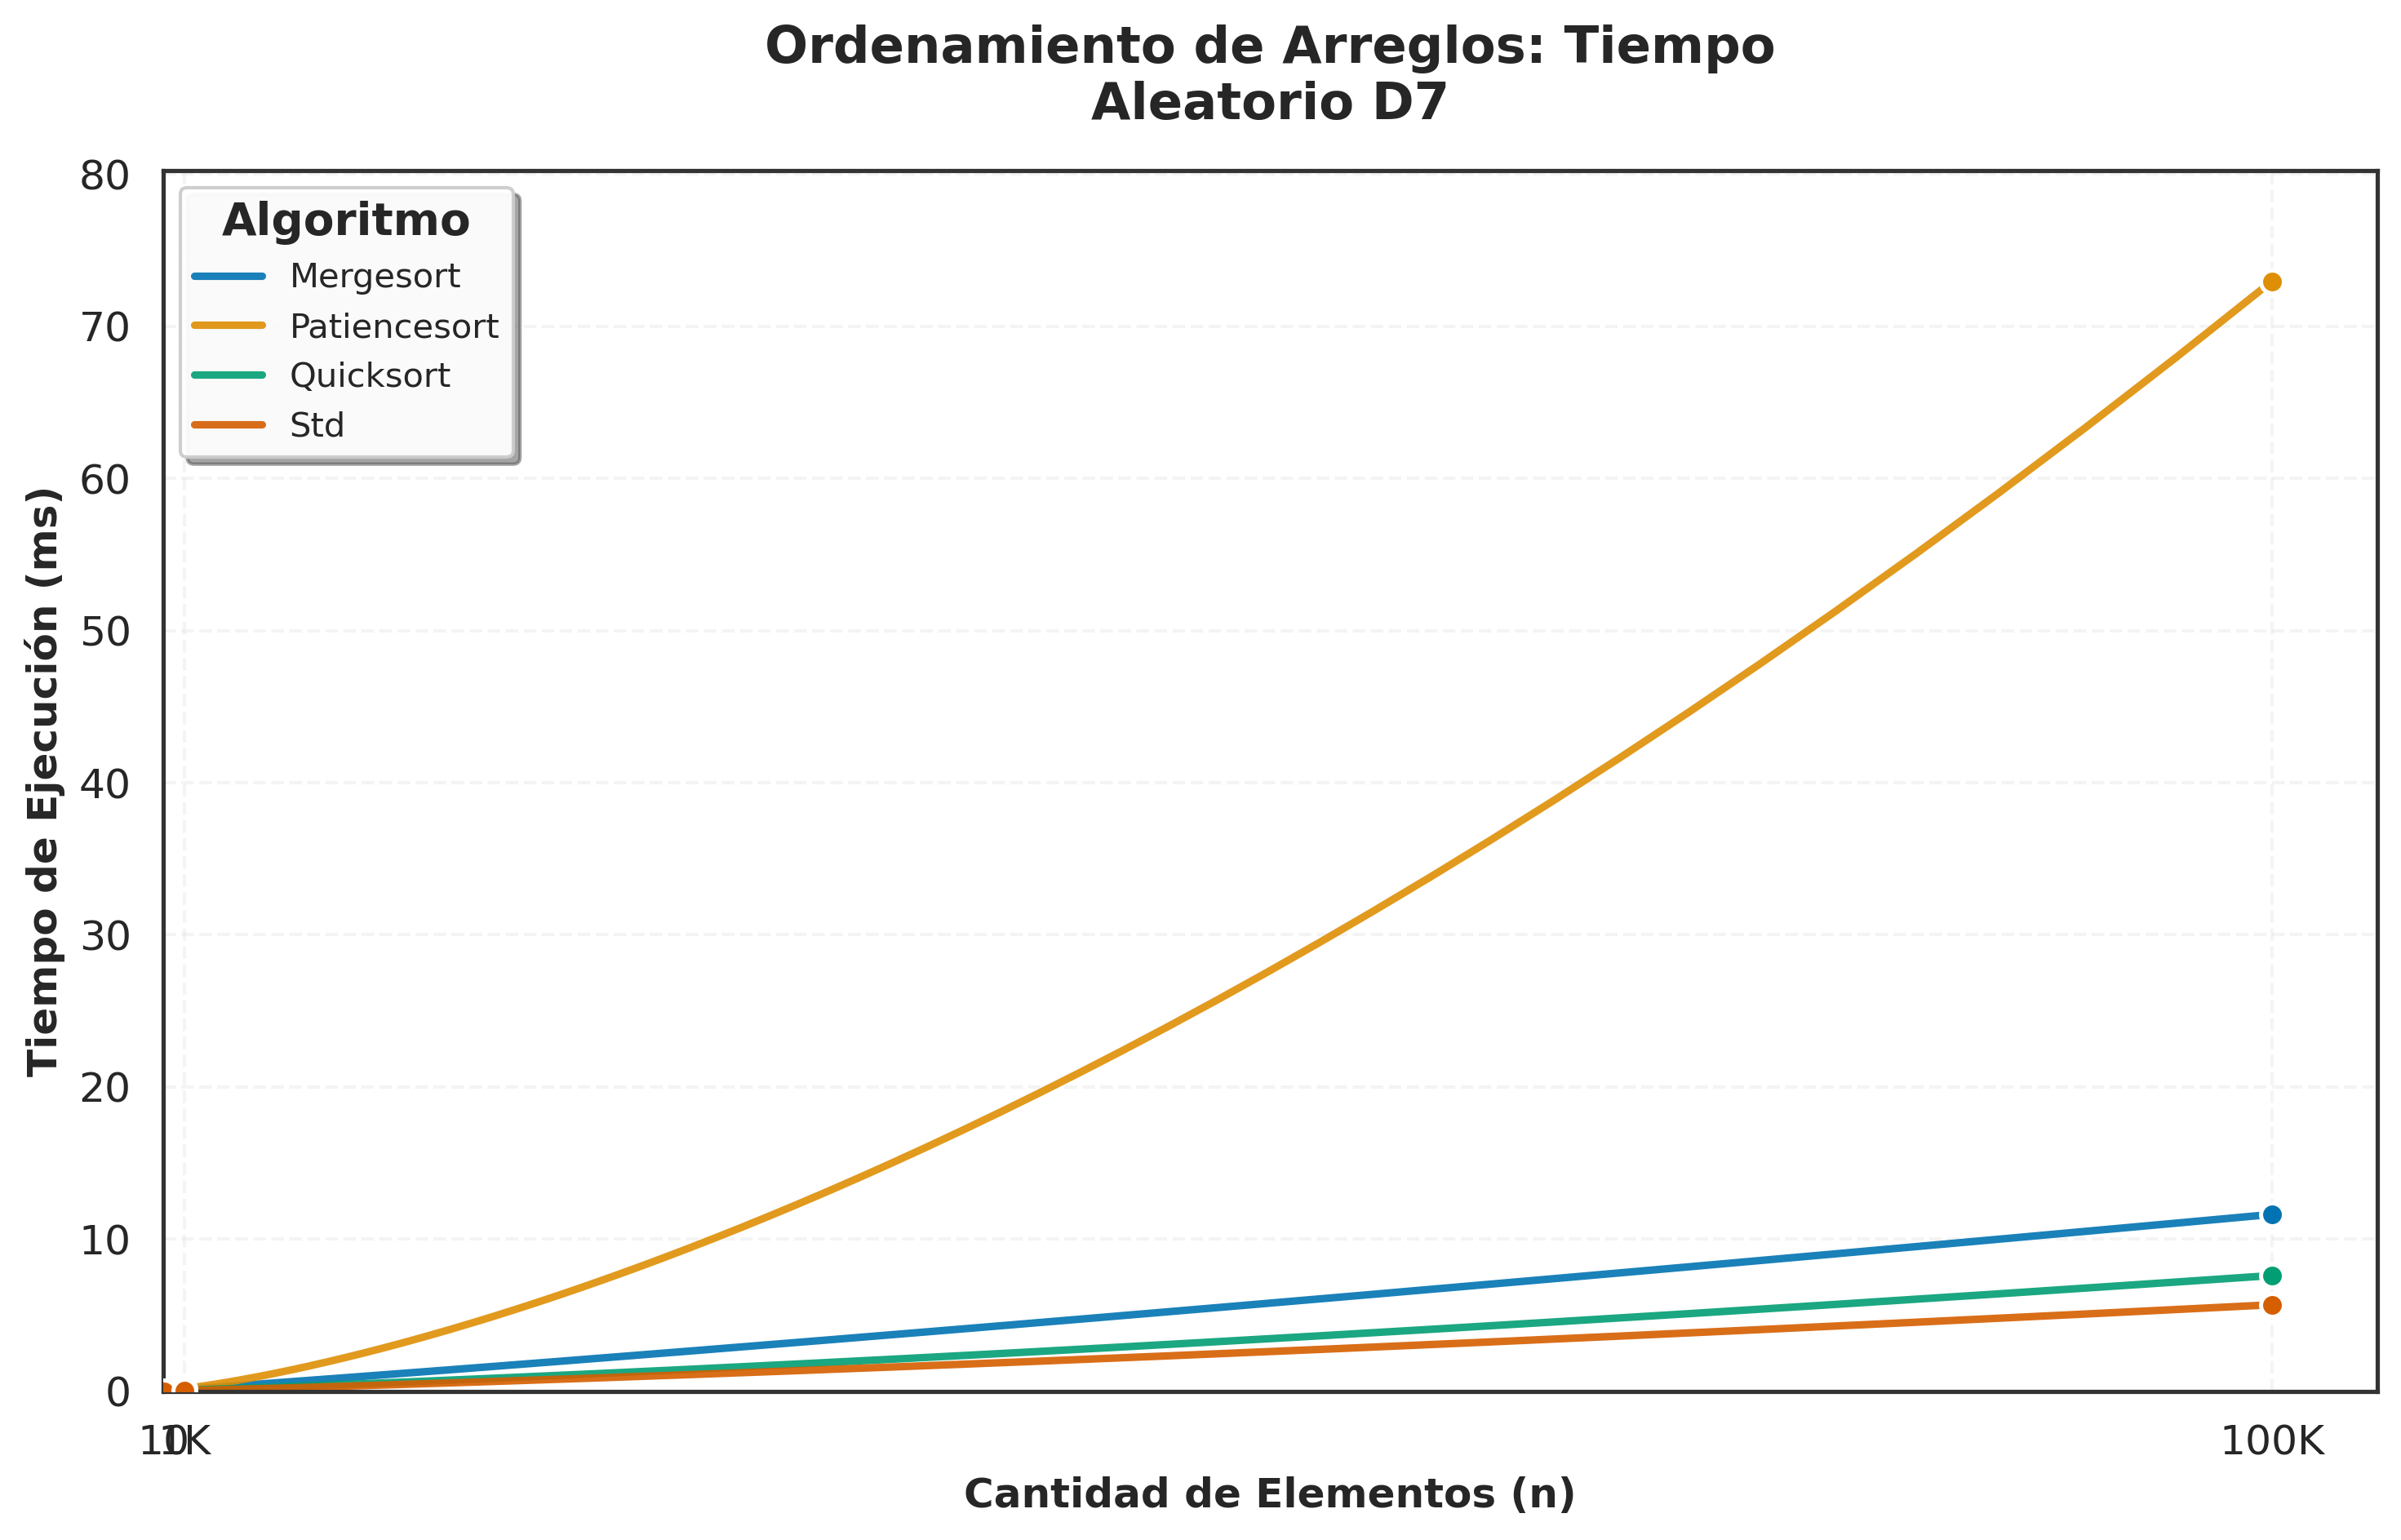
\includegraphics[width=\linewidth]{../code/sorting/data/plots/tiempo_aleatorio_D7.png}
    \caption{Tiempo de ejecución, arreglos aleatorios (D7).}
    \label{fig:sort_aleatorio}
\end{minipage}\hfill
\begin{minipage}[t]{0.31\textwidth}
    \centering
    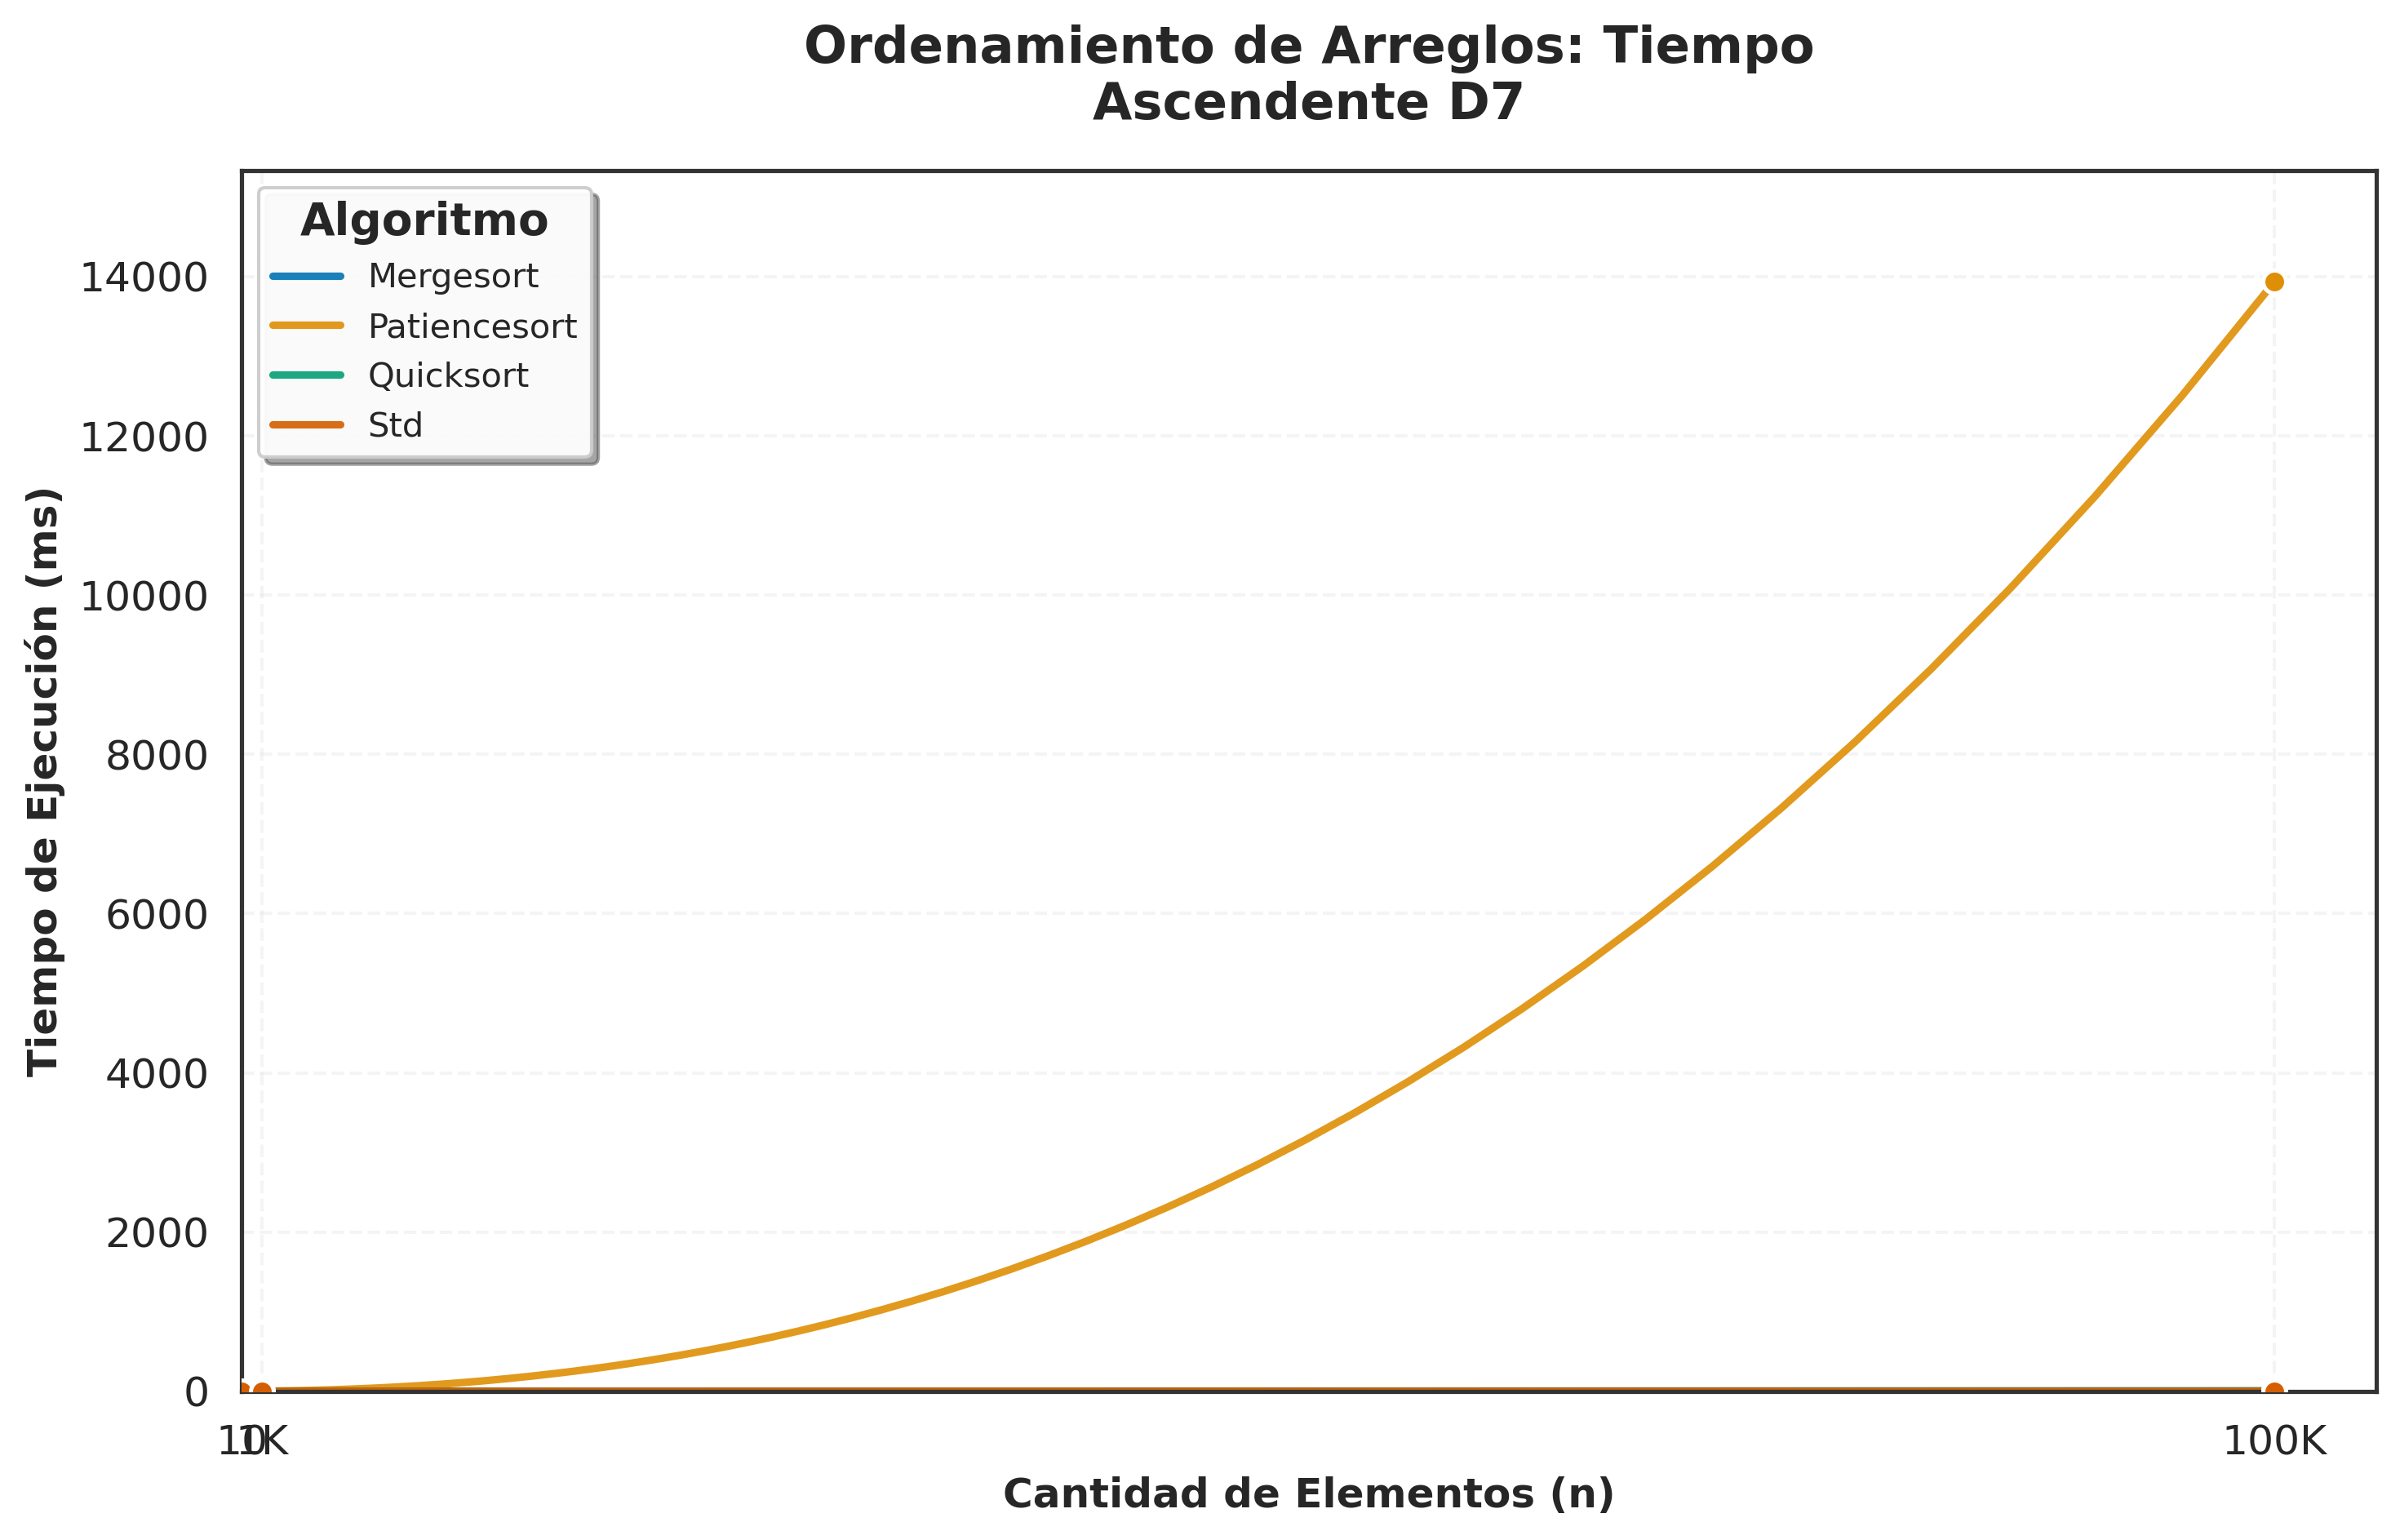
\includegraphics[width=\linewidth]{../code/sorting/data/plots/tiempo_ascendente_D7.png}
    \caption{Tiempo de ejecución, arreglos ascendentes (D7).}
    \label{fig:sort_asc}
\end{minipage}\hfill
\begin{minipage}[t]{0.31\textwidth}
    \centering
    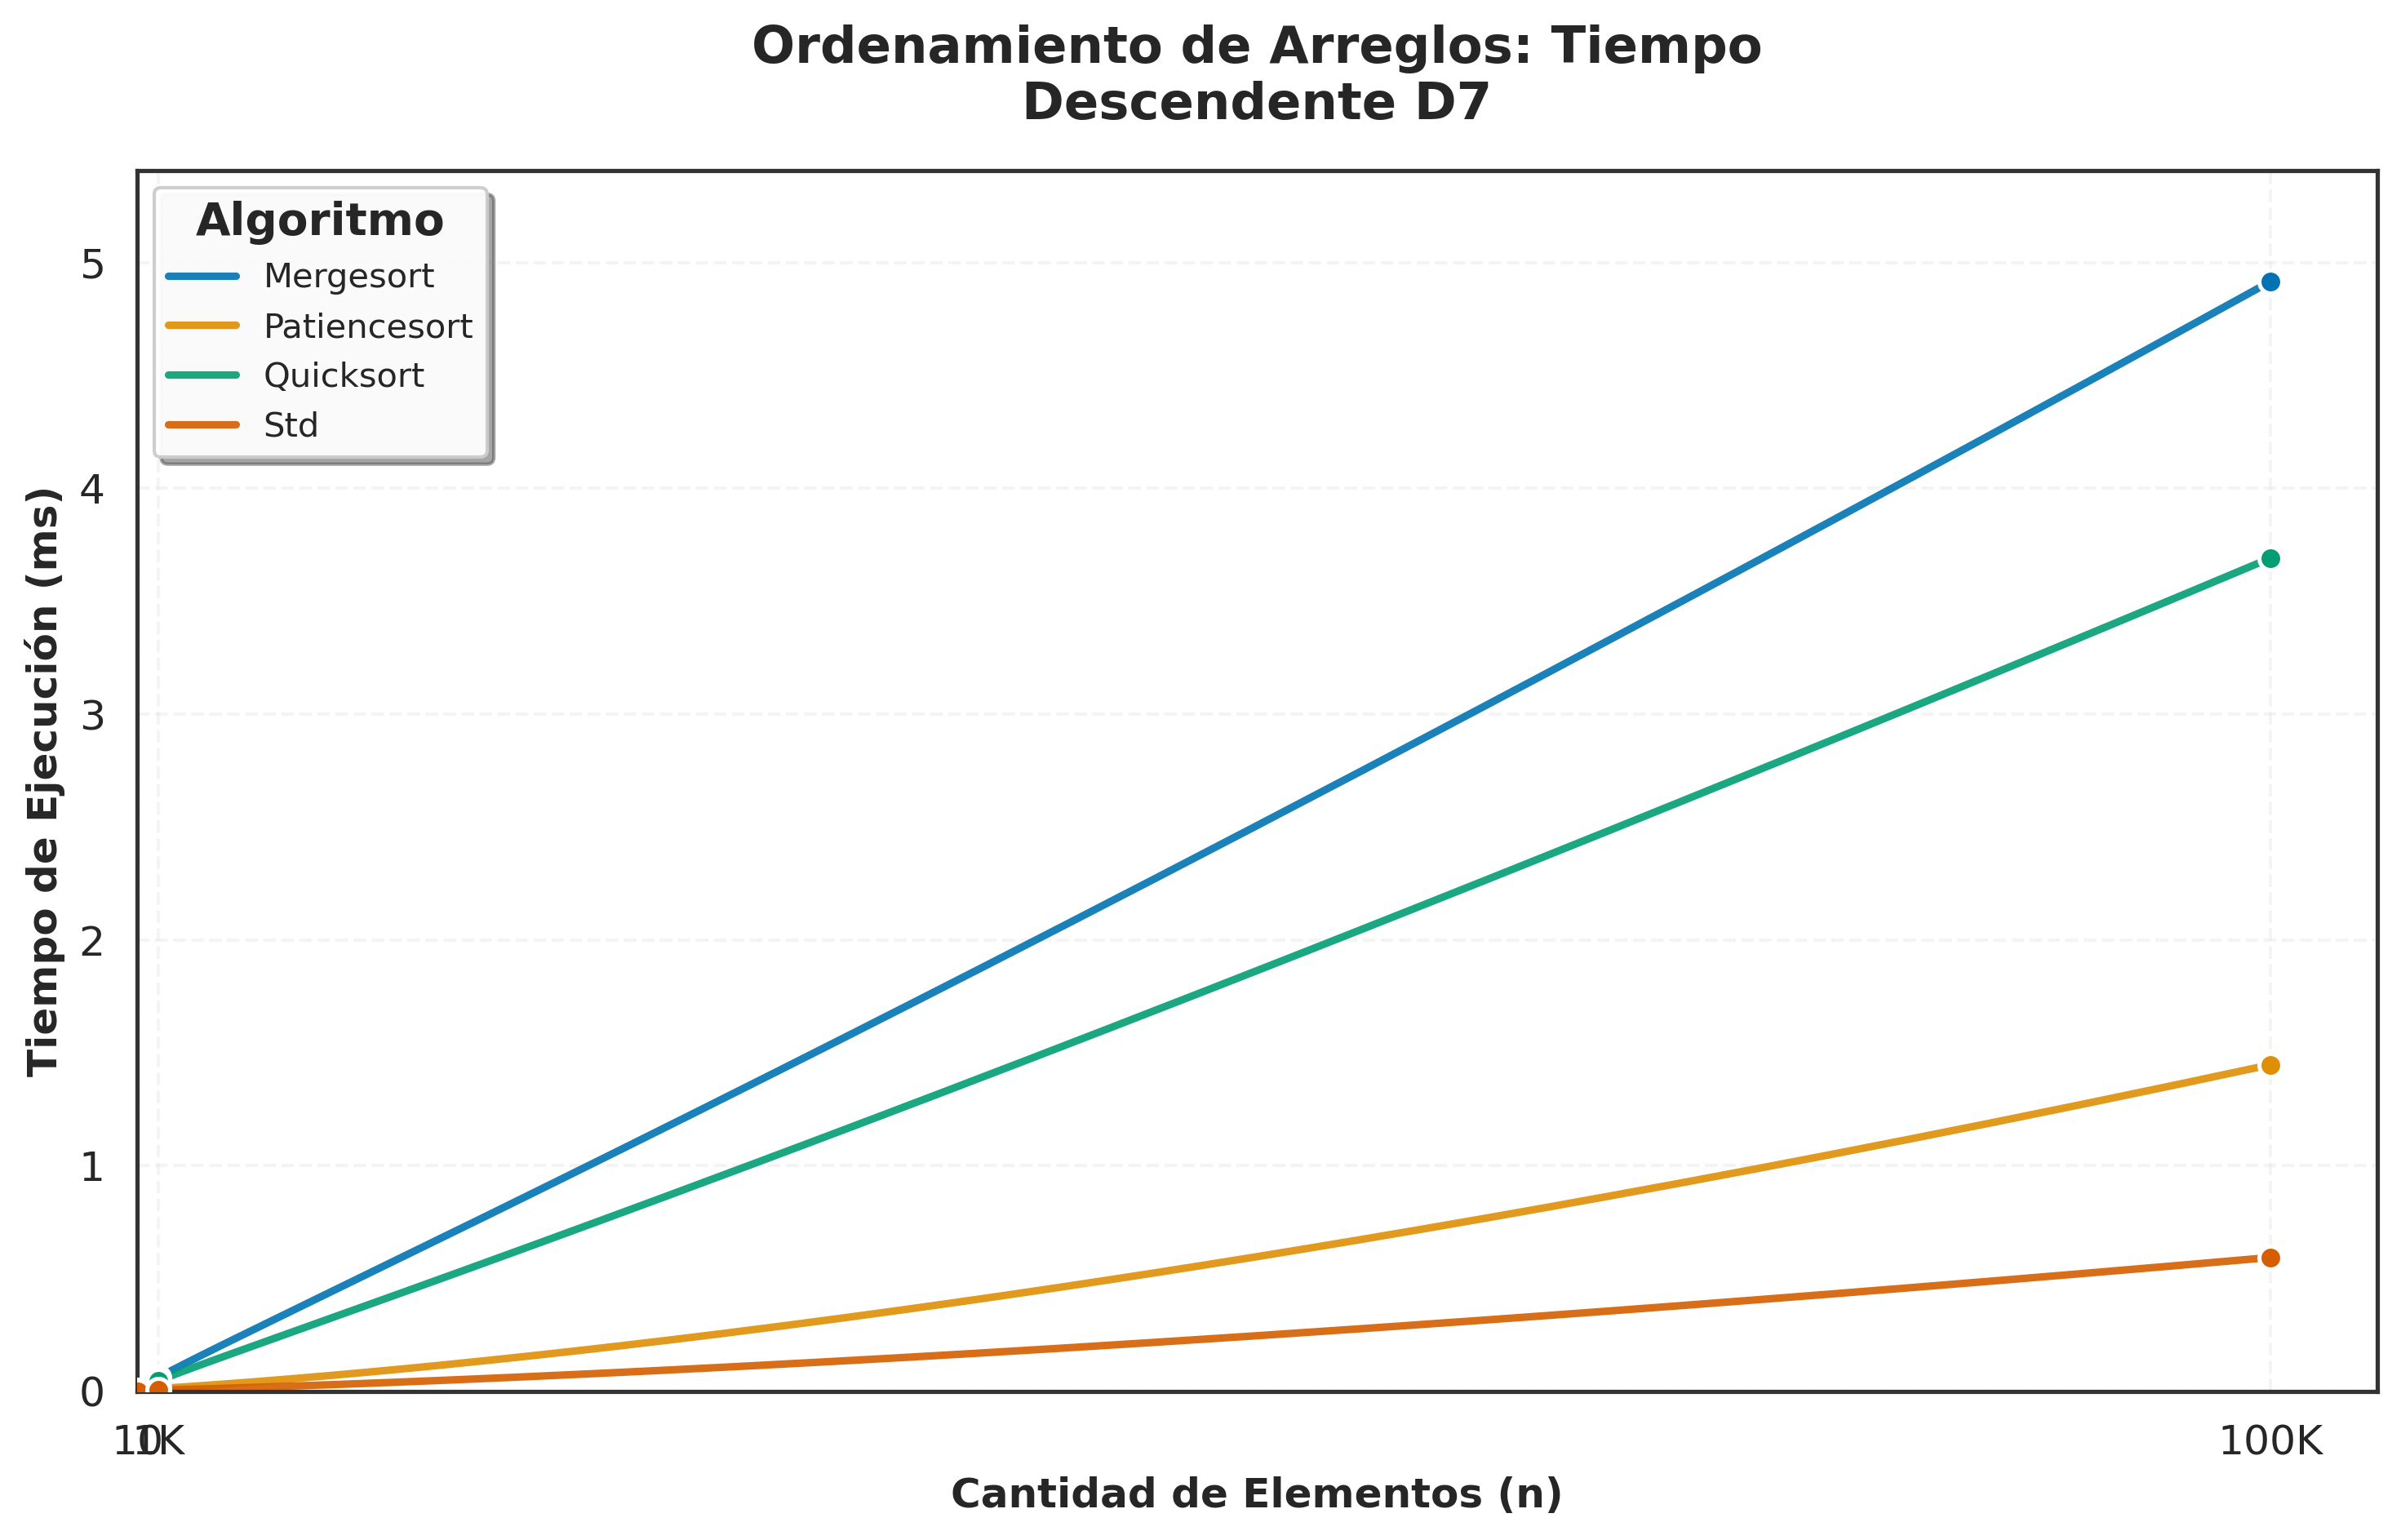
\includegraphics[width=\linewidth]{../code/sorting/data/plots/tiempo_descendente_D7.png}
    \caption{Tiempo de ejecución, arreglos descendentes (D7).}
    \label{fig:sort_des}
\end{minipage}\\[6pt]
\begin{minipage}[t]{0.31\textwidth}
    \centering
    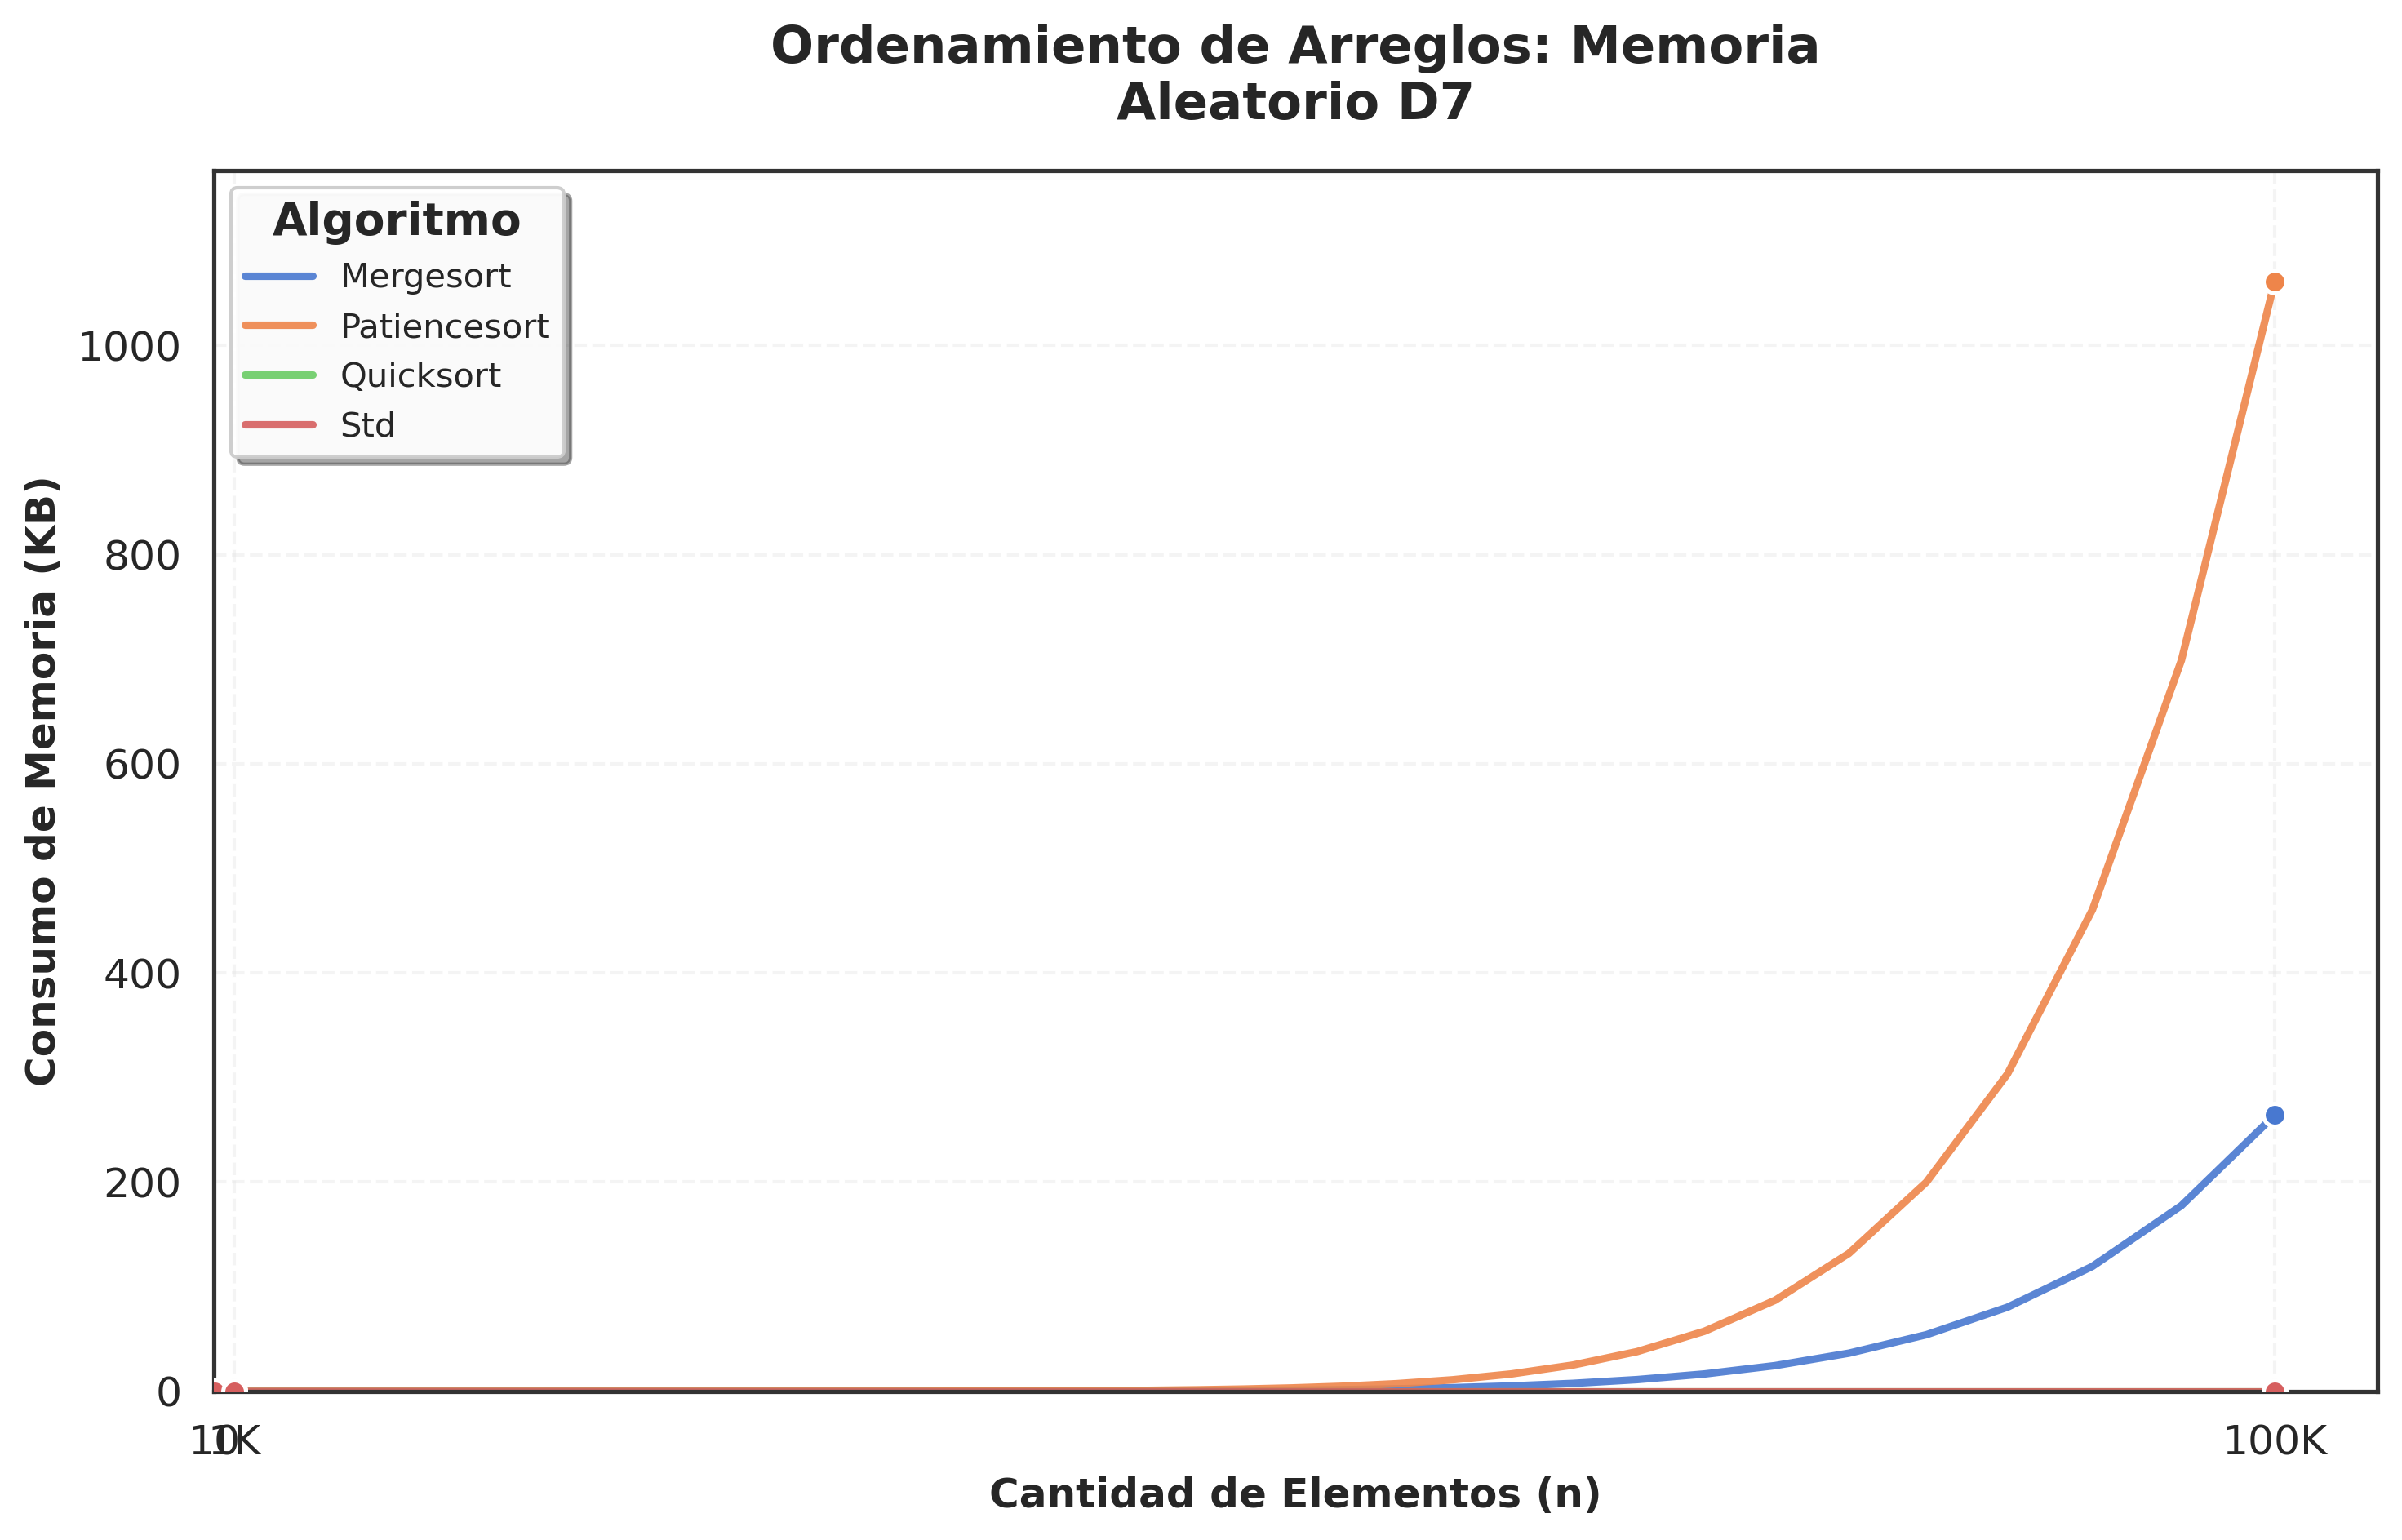
\includegraphics[width=\linewidth]{../code/sorting/data/plots/memoria_aleatorio_D7.png}
    \caption{Consumo de memoria, arreglos aleatorios (D7).}
    \label{fig:sort_mem}
\end{minipage}\hfill
\begin{minipage}[t]{0.31\textwidth}
    \centering
    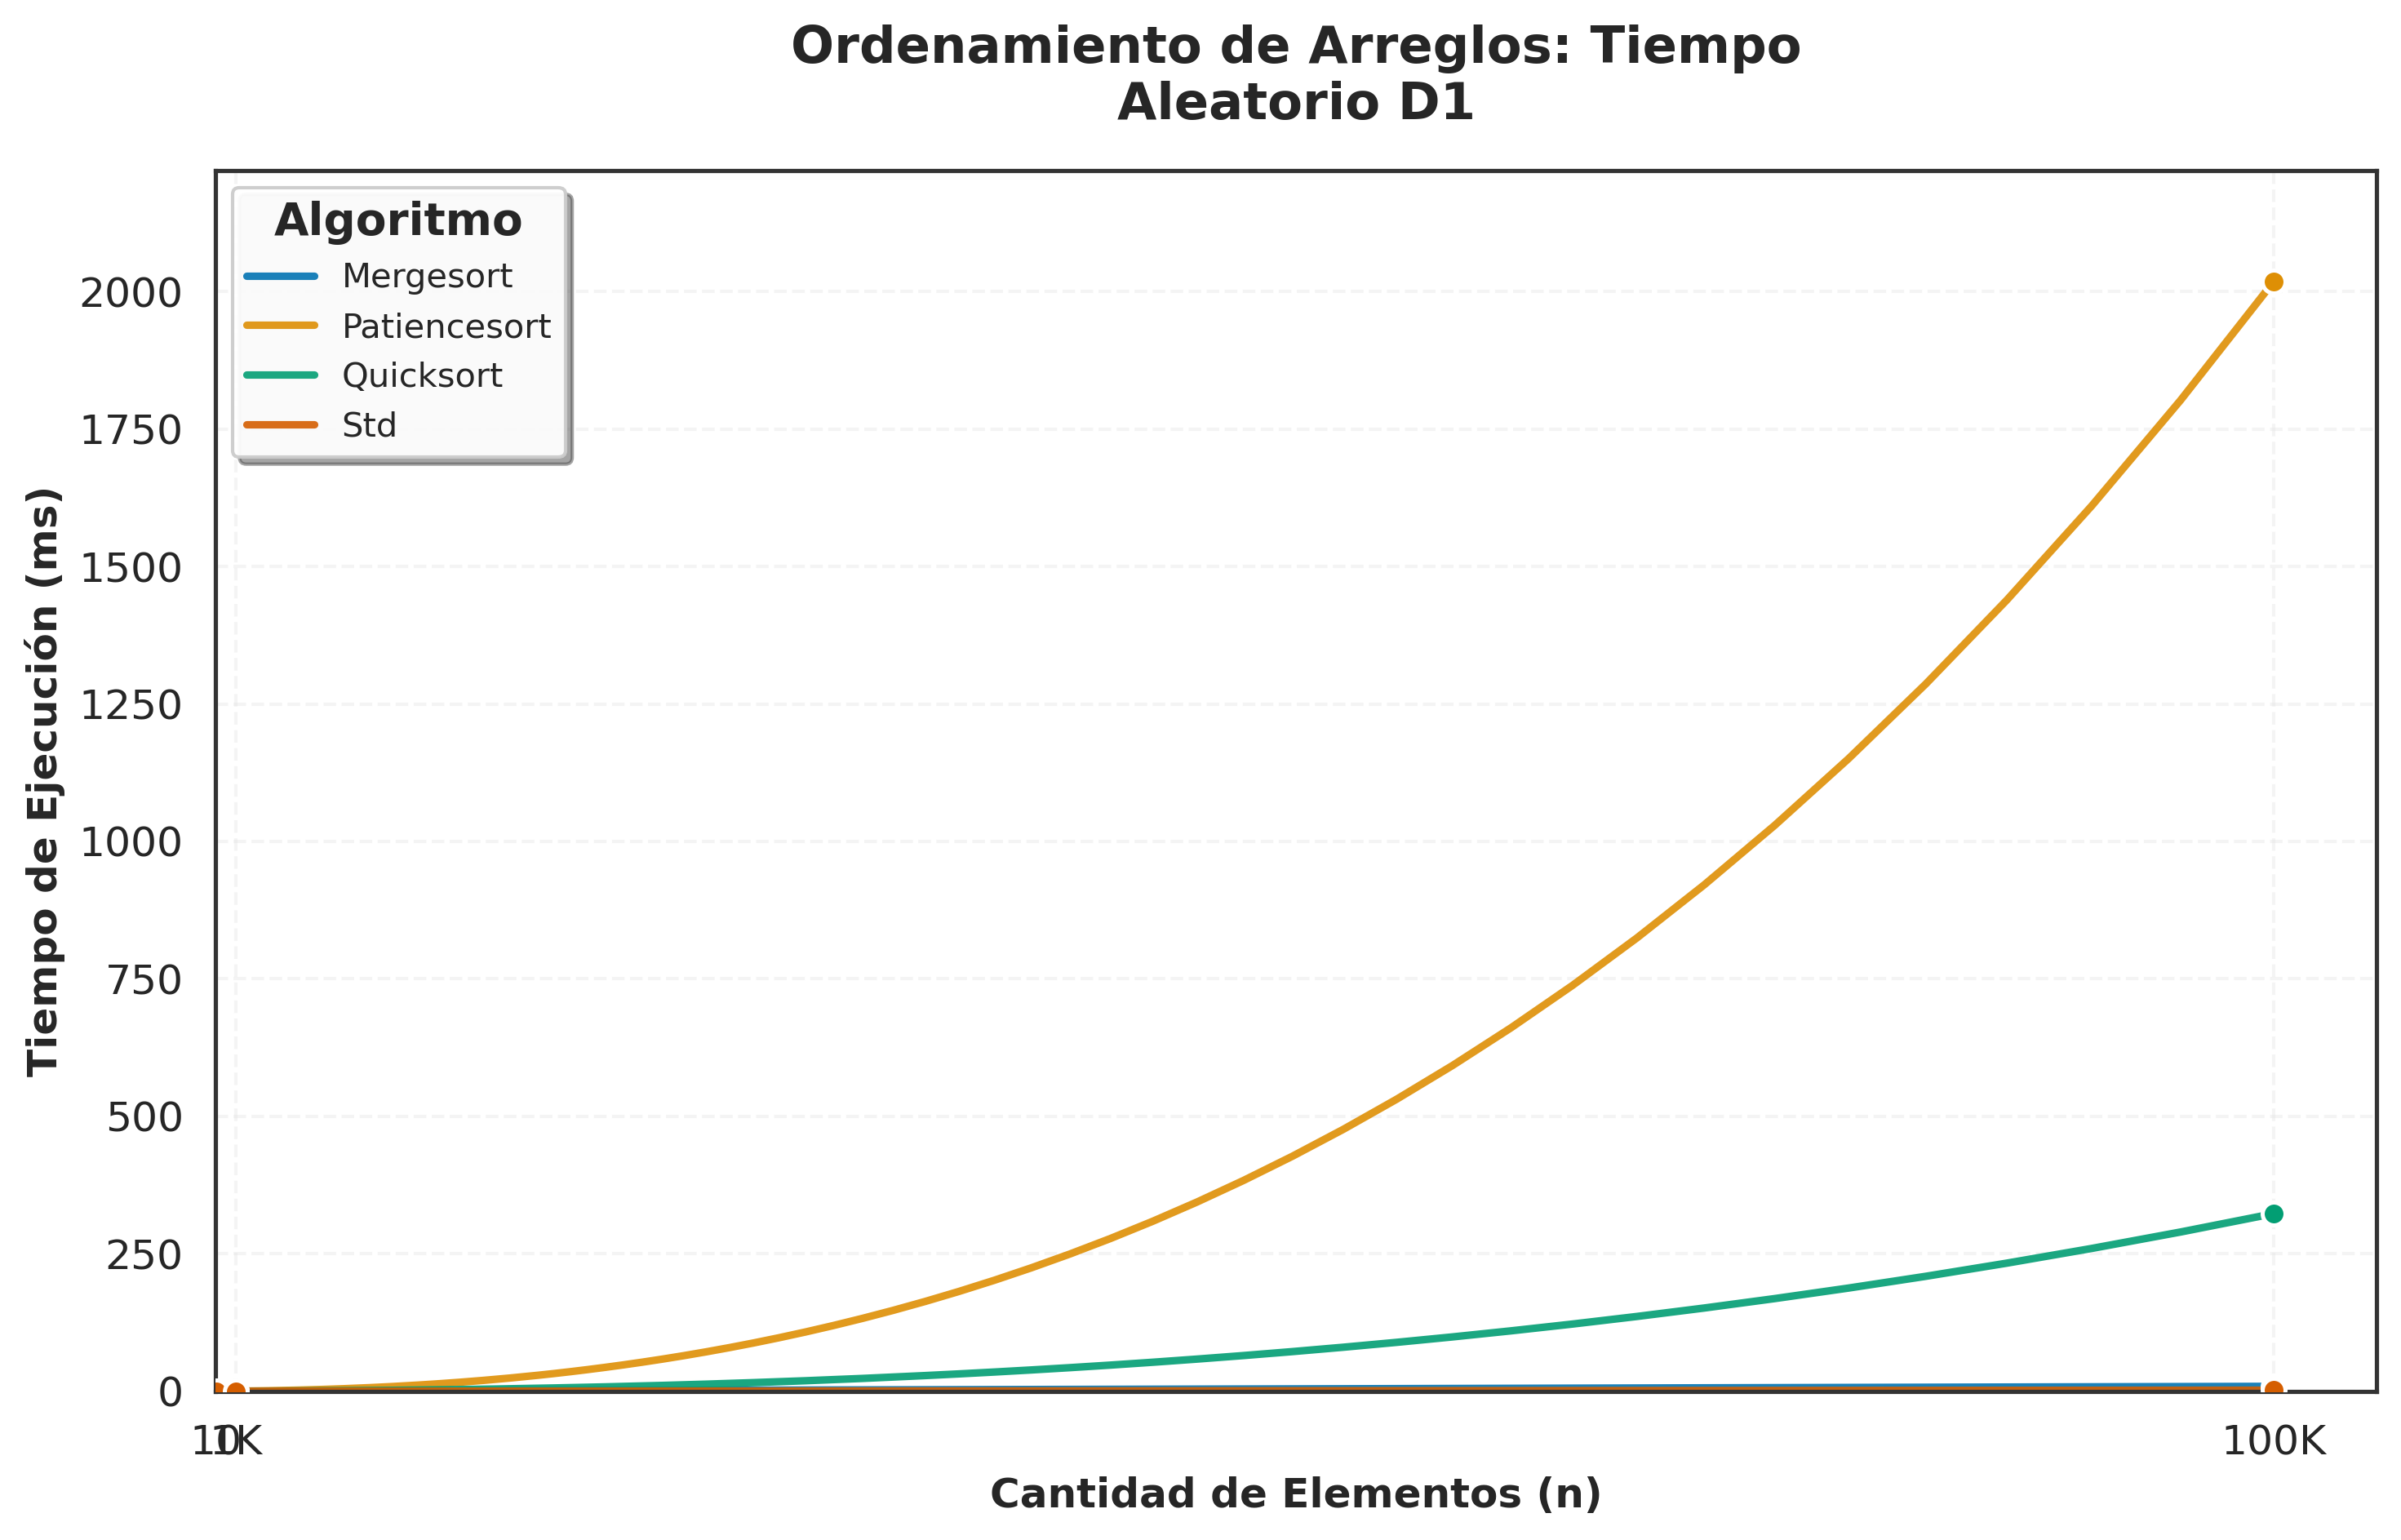
\includegraphics[width=\linewidth]{../code/sorting/data/plots/tiempo_aleatorio_D1.png}
    \caption{Tiempo de ejecución, arreglos aleatorios (D1).}
    \label{fig:sort_aleatorio_D1}
\end{minipage}\hfill
\begin{minipage}[t]{0.31\textwidth}
    \centering
    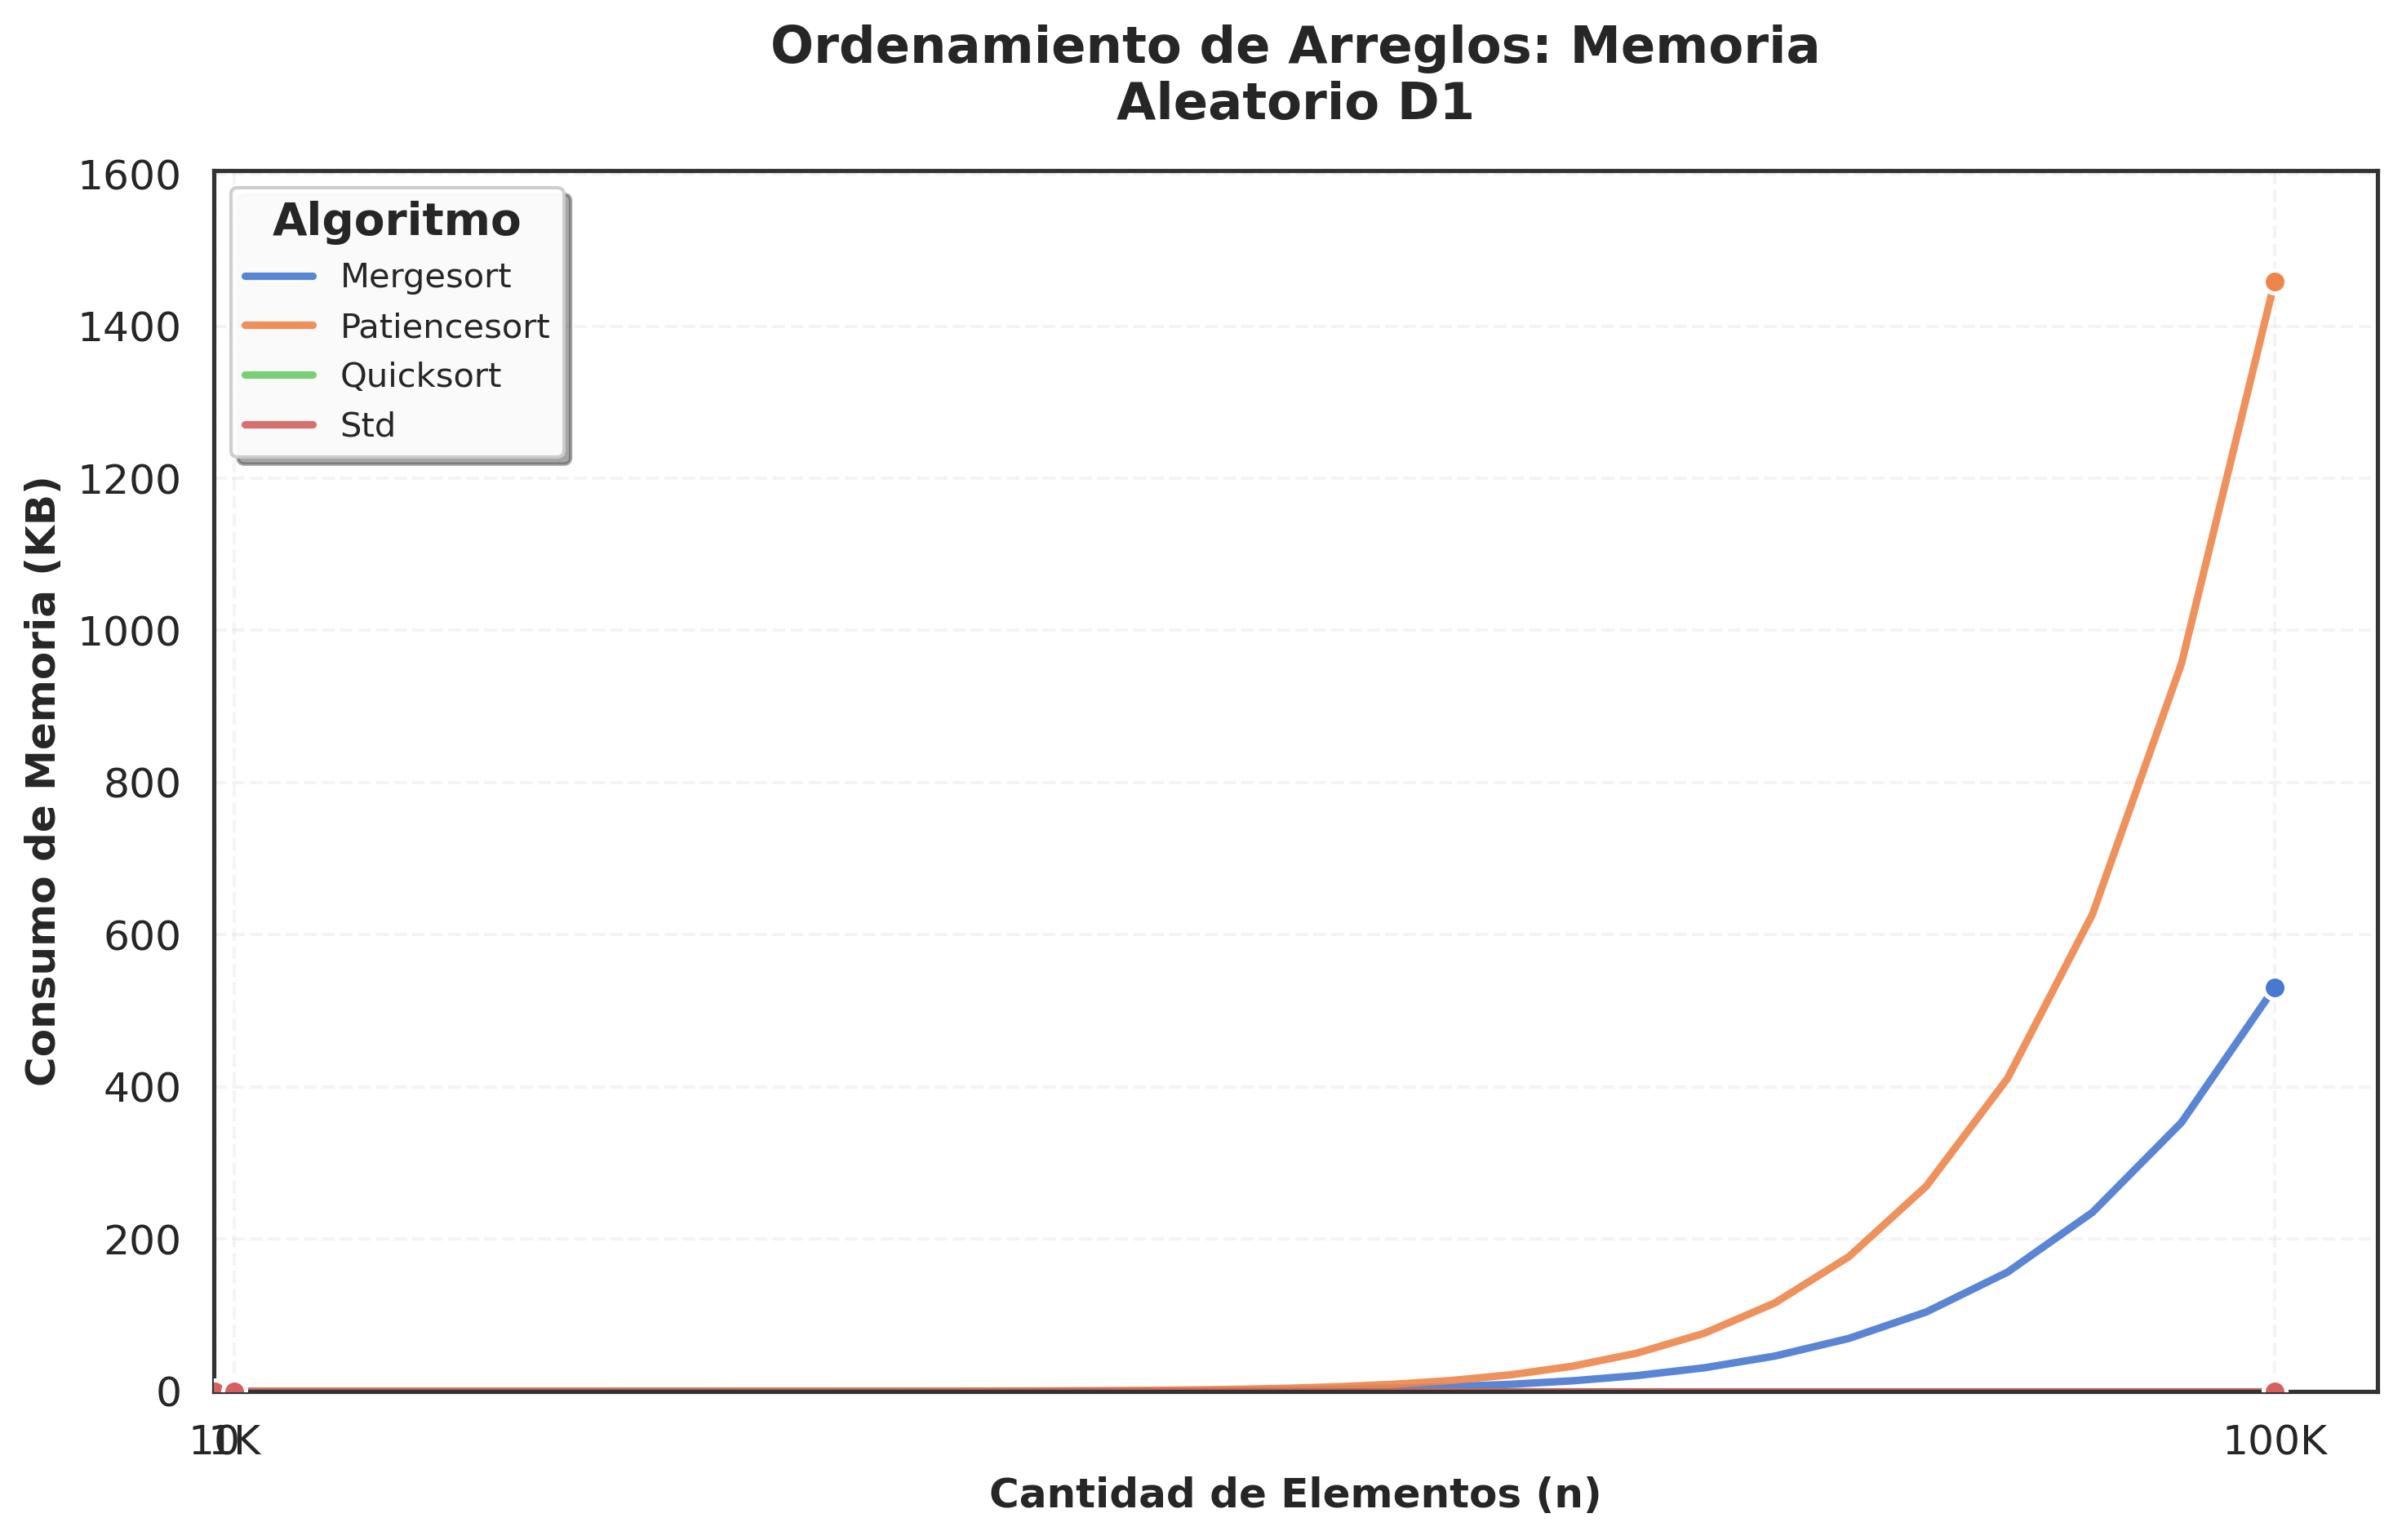
\includegraphics[width=\linewidth]{../code/sorting/data/plots/memoria_aleatorio_D1.png}
    \caption{Consumo de memoria, arreglos aleatorios (D1).}
    \label{fig:sort_mem_D1}
\end{minipage}
\end{figure}


En la Figura 1, el orden fue
$std::sort$ ($\approx 6$ ms) $<$ $QuickSort$ ($\approx 8$ ms) $<$
$MergeSort$ ($\approx 12$ ms) $<$ $PatienceSort$ ($\approx 80$ ms). Los tres
primeros comparten $O(n \log n)$, por lo tanto la diferencia radica simplemente en el valor de la constante que multiplica la complejidad, la cual está dada por una mayor cantidad de operaciones elementales. Por otro lado, podemos notar claramente el rápido crecimiento de $PatienceSort$. 




En la Figura 2 pasa algo interesante, se puede ver claramente lo que sucede en el peor caso de un algoritmo con complejidad $O(n^2)$. Esto se debe principalmente a que se debe crear una pila por elemento y realizar búsquedas lineales constantemente.



En la Figura 3 podemos notar que este caso es mucho más favorable para $PatienceSort$, debido a que cada elemento es mayor o igual que el siguiente que se prueba, utilizando solo una pila y superando a $QuickSort$ y $MergeSort$. Esto nos enseña que no hay un caso general para medir el tiempo de un algoritmo con complejidad temporal diferente de $\Theta ($f(n)$)$.


En la Figura 4 se puede observar que el consumo de memoria es coherente con la complejidad teórica, donde $MergeSort$ y $PatienceSort$ crecen de forma
proporcional a $O(n)$, el primero por los vectores temporales que va generando en las recursiones y el segundo debido a las pilas que va generando. Por otro lado $QuickSort$ y $std::sort$ prácticamente no usan memoria, esto se debe a que teóricamente $std::sort$ es in-place y $QuickSort$ en teoría no es in-place si se implementa de manera recursiva, porque en cada nivel de la recursión apila el marco de llamadas en el stack referente a los punteros, por lo que el uso de memoria debería crecer con la profundidad (O(logn) con pivote aleatorio), pero debido a la forma en la que se mide la memoria con VmHWM y a que para n = $10^7$ consume menos de 4KB, no se detecta prácticamente nada.

En la Figura 5 podemos observar que el tiempo de $PatienceSort$ aumenta drásticamente comparado a lo que sucedía en $D7$. Esto se debe principalmente a que como existen solo diez valores posibles, los arreglos más grandes tienen muchos elementos duplicados y como la condición de PatienceSort es buscar elementos estrictamente menores, hace que los duplicados no se puedan almacenar en la misma pila, lo que obliga a crear una pila nueva constantemente y realizar muchas búsquedas lineales.



En la Figura 6 podemos notar la consecuencia directa de lo mencionado anteriormente, $PatienceSort$ utiliza una mayor cantidad de memoria debido a la necesidad de manejar con pilas los elementos duplicados, $MergeSort$ mantiene su curva y $std::sort$ consume ligeramente más memoria que en D7 debido a la existencia de los elementos duplicados, lo que produce una recursión más profunda.

\subsection{Multiplicación de matrices cuadradas}
Al igual que para los algoritmos de ordenamiento, en este caso es importante conocer las complejidades teóricas y prácticas de los algoritmos de multiplicación de matrices $Naive$ y $Strassen$.


\begin{table}[H]
\centering
\label{tab:complejidades_mat}
\begin{tabular}{|l|c|c|c|l|}
\hline
\textbf{Algoritmo} & \textbf{C. temporal teórica} & \textbf{C. temporal impl.} & \textbf{C. espacial} & \textbf{Fuente} \\ \hline
Naive & $O(N^3)$ & $O(N^3)$ & $O(N^2)$ & 
\href{https://www.studymite.com/cpp/examples/multiply-two-matrices-in-cpp}{Studymite} \\ \hline
Strassen & $O(N^{2.81})$ & $O(N^{2.81})$ & $O(N^2)$ &
\href{https://github.com/psakoglou/Strassen-Algorithm-Simulation-and-Asymptotic-Efficiency-CPP}{GitHub (psakoglou)} \\ \hline
\end{tabular}
\end{table}


A continuación, el análisis de gráficos:


\begin{figure}[H]
\centering
\begin{minipage}[t]{0.31\textwidth}
    \centering
    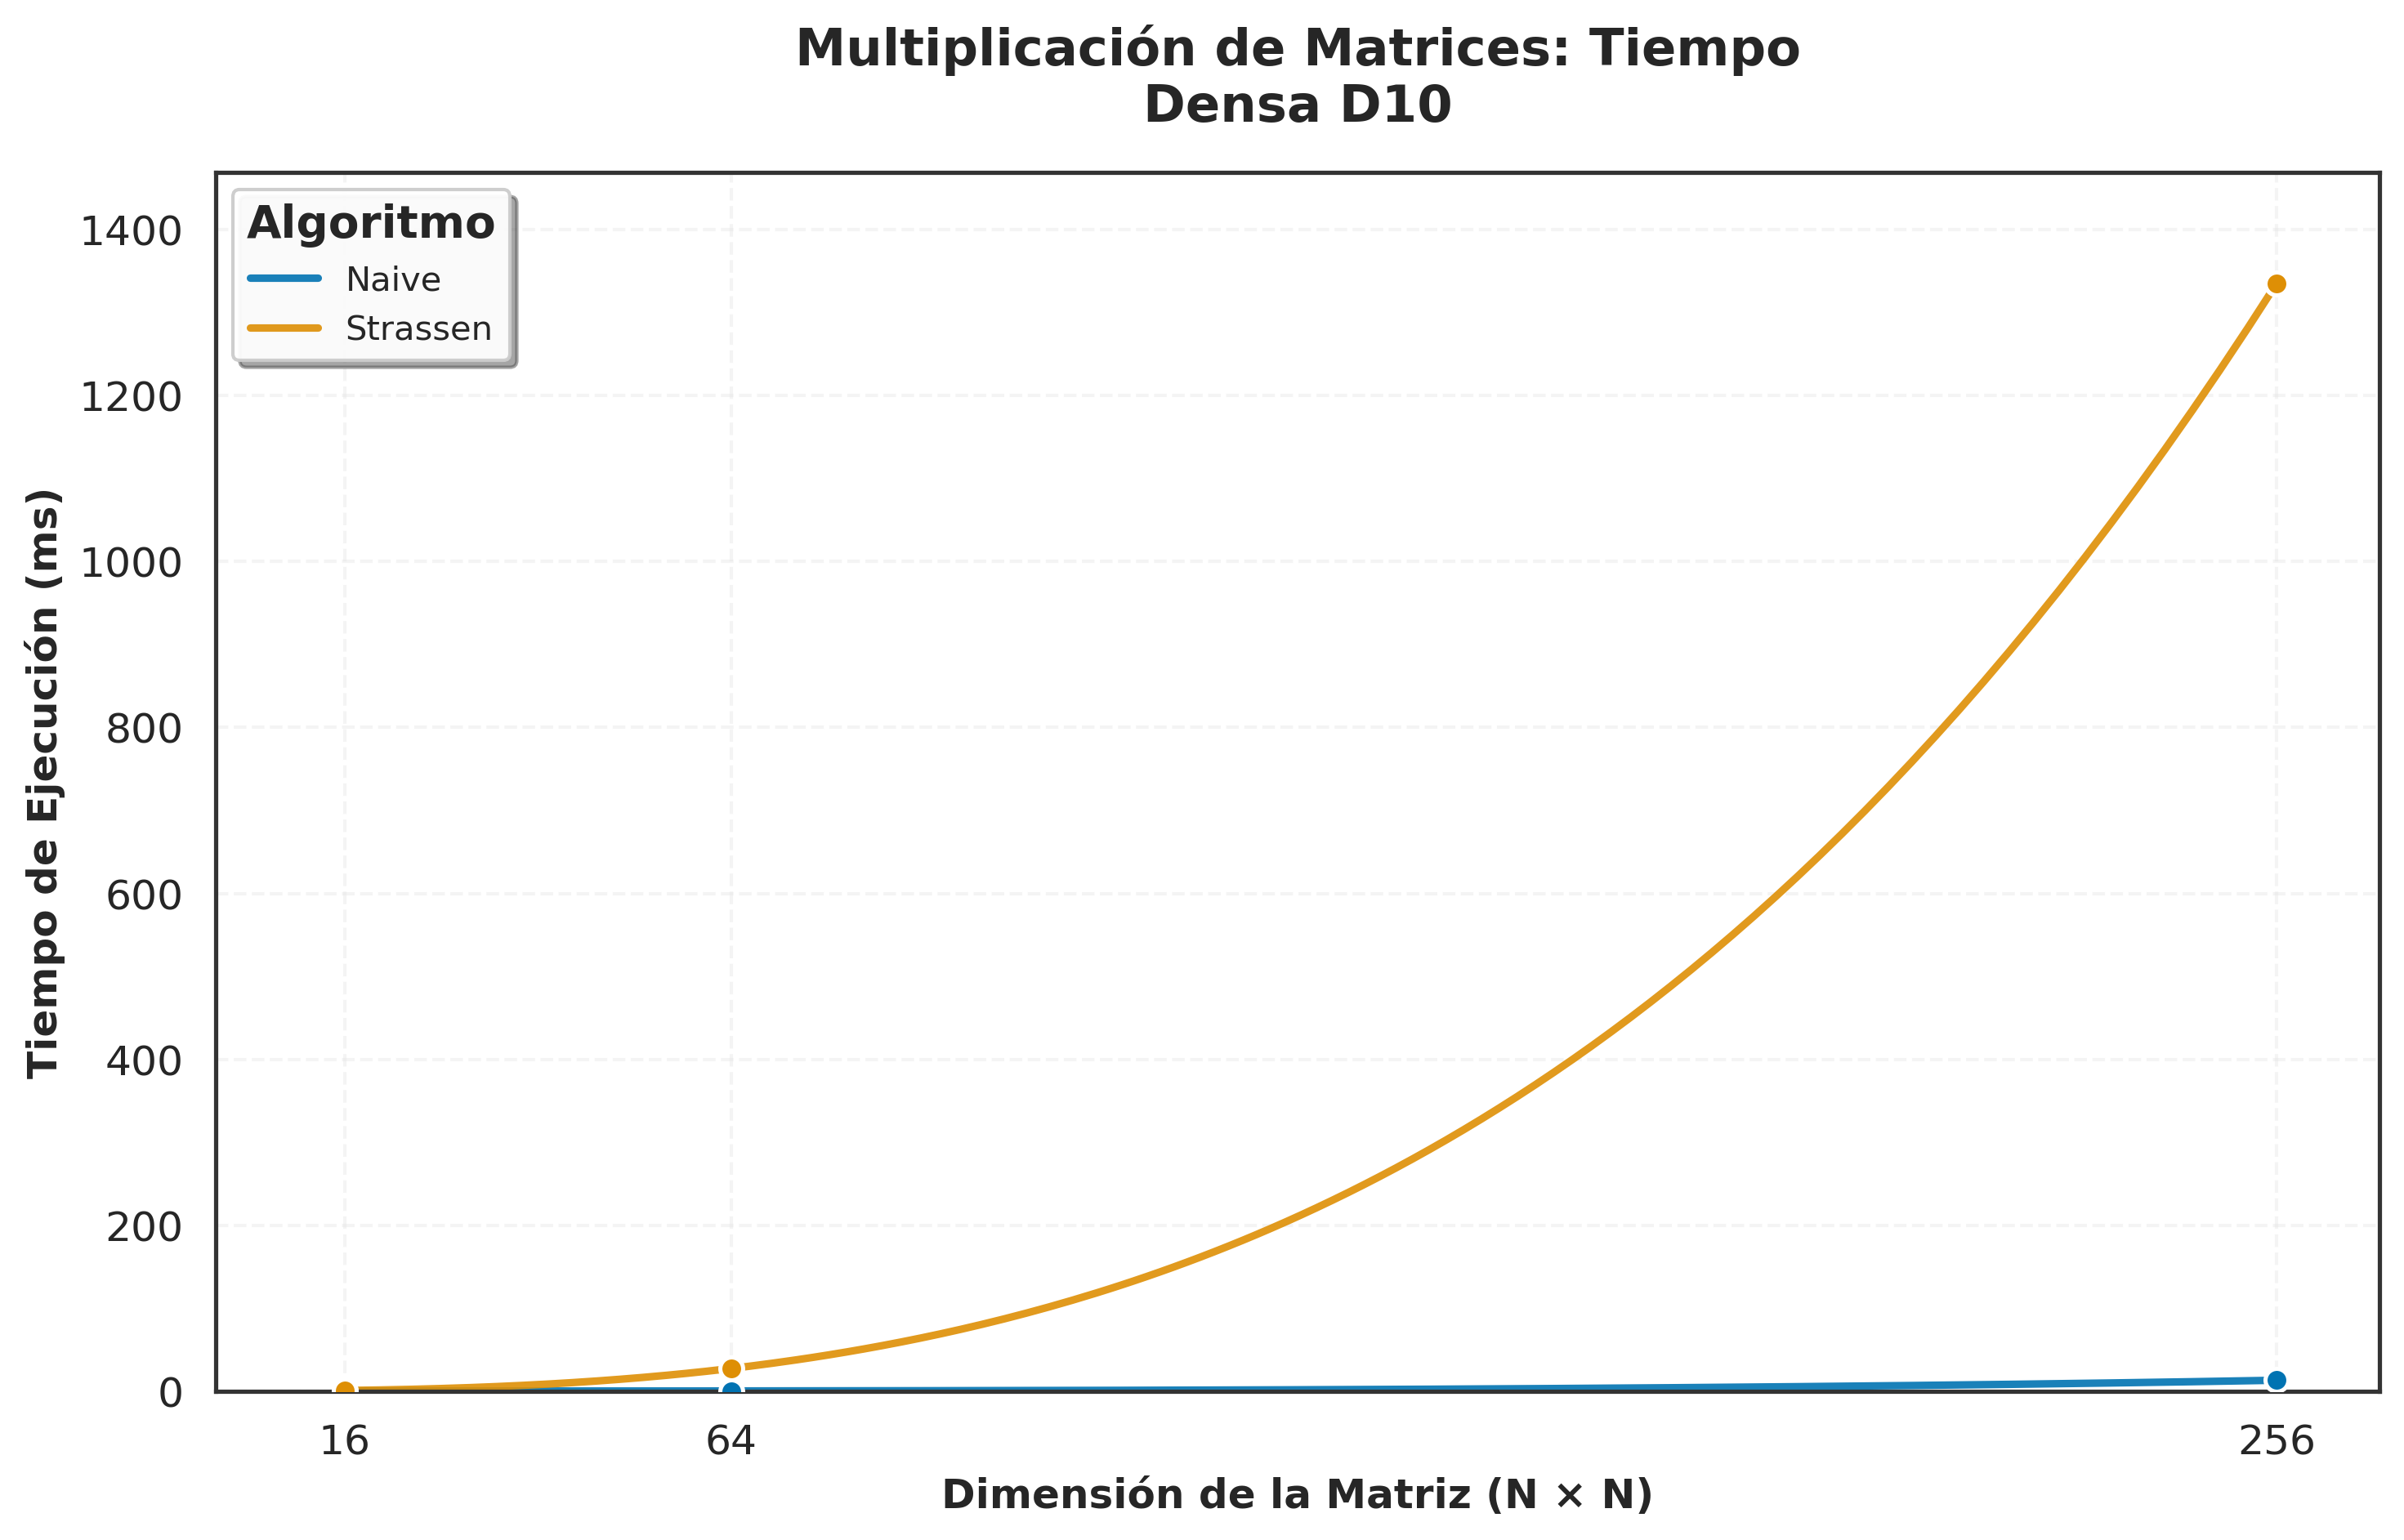
\includegraphics[width=\linewidth]{../code/matrix_multiplication/data/plots/tiempo_densa_D10.png}
    \caption{Tiempo, matrices densas (D10).}
    \label{fig:mat_tiempo}
\end{minipage}\hfill
\begin{minipage}[t]{0.31\textwidth}
    \centering
    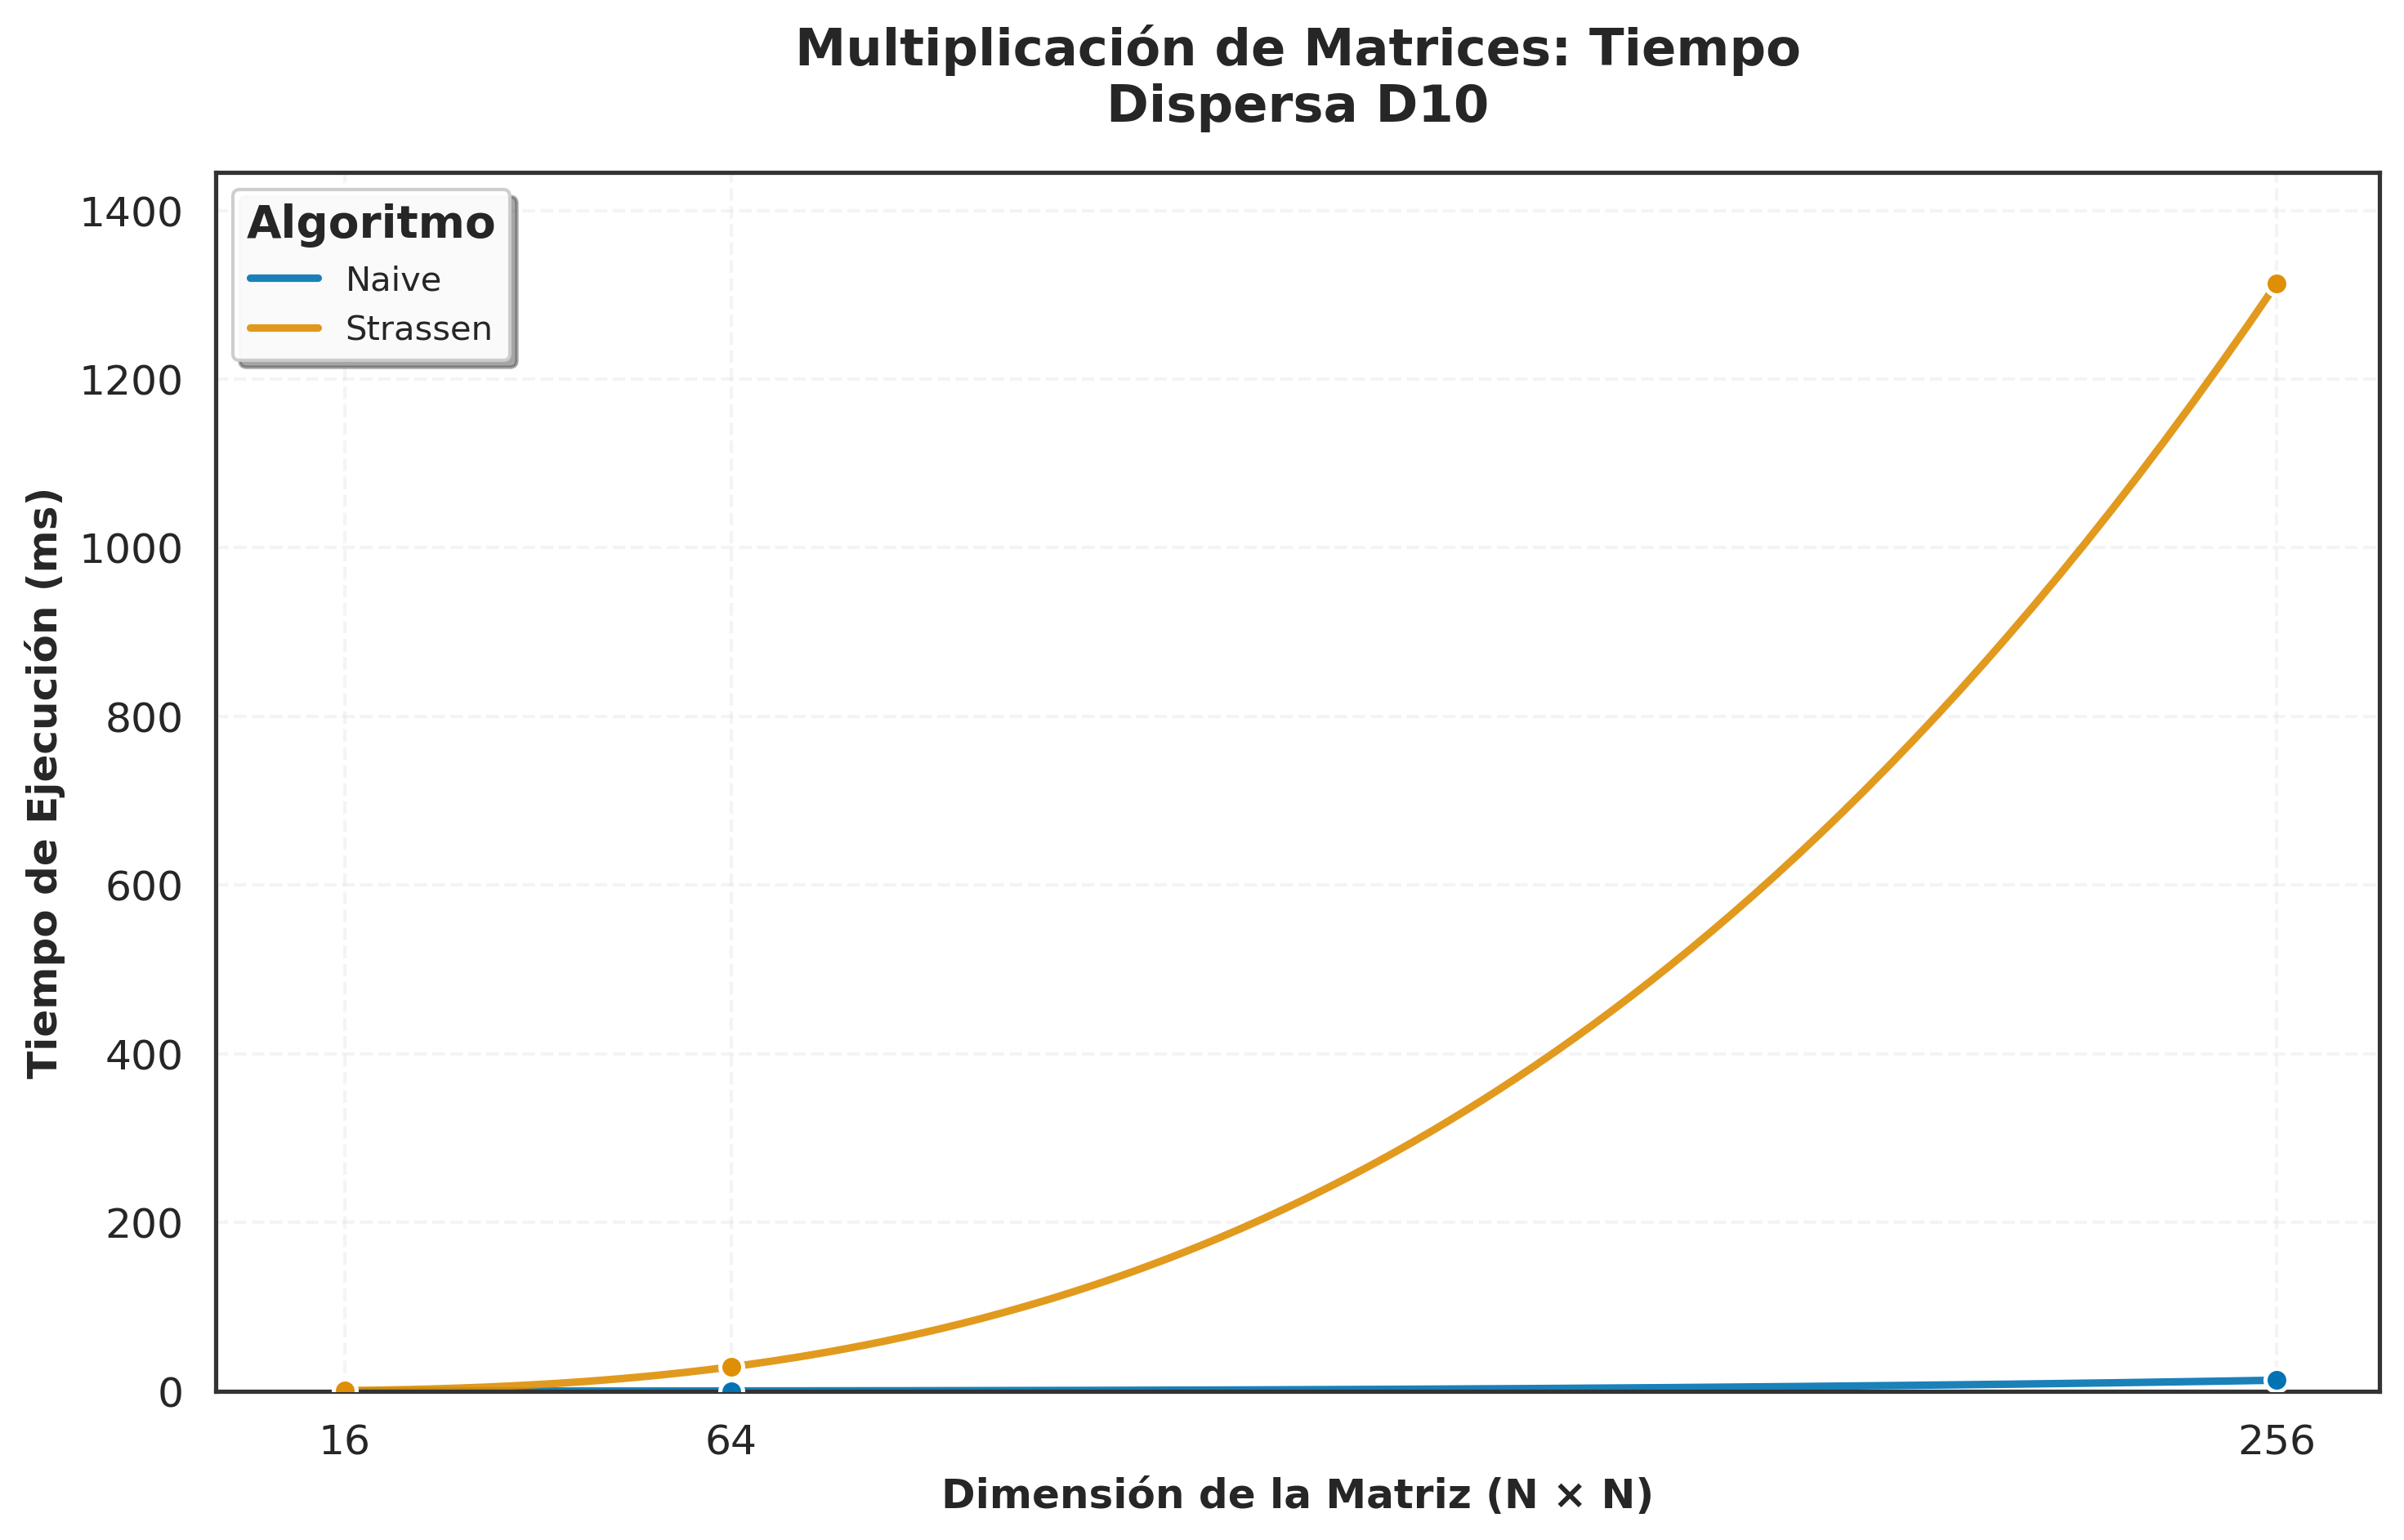
\includegraphics[width=\linewidth]{../code/matrix_multiplication/data/plots/tiempo_dispersa_D10.png}
    \caption{Tiempo, matrices dispersas (D10).}
    \label{fig:mat_tiempo_disp10}
\end{minipage}\hfill
\begin{minipage}[t]{0.31\textwidth}
    \centering
    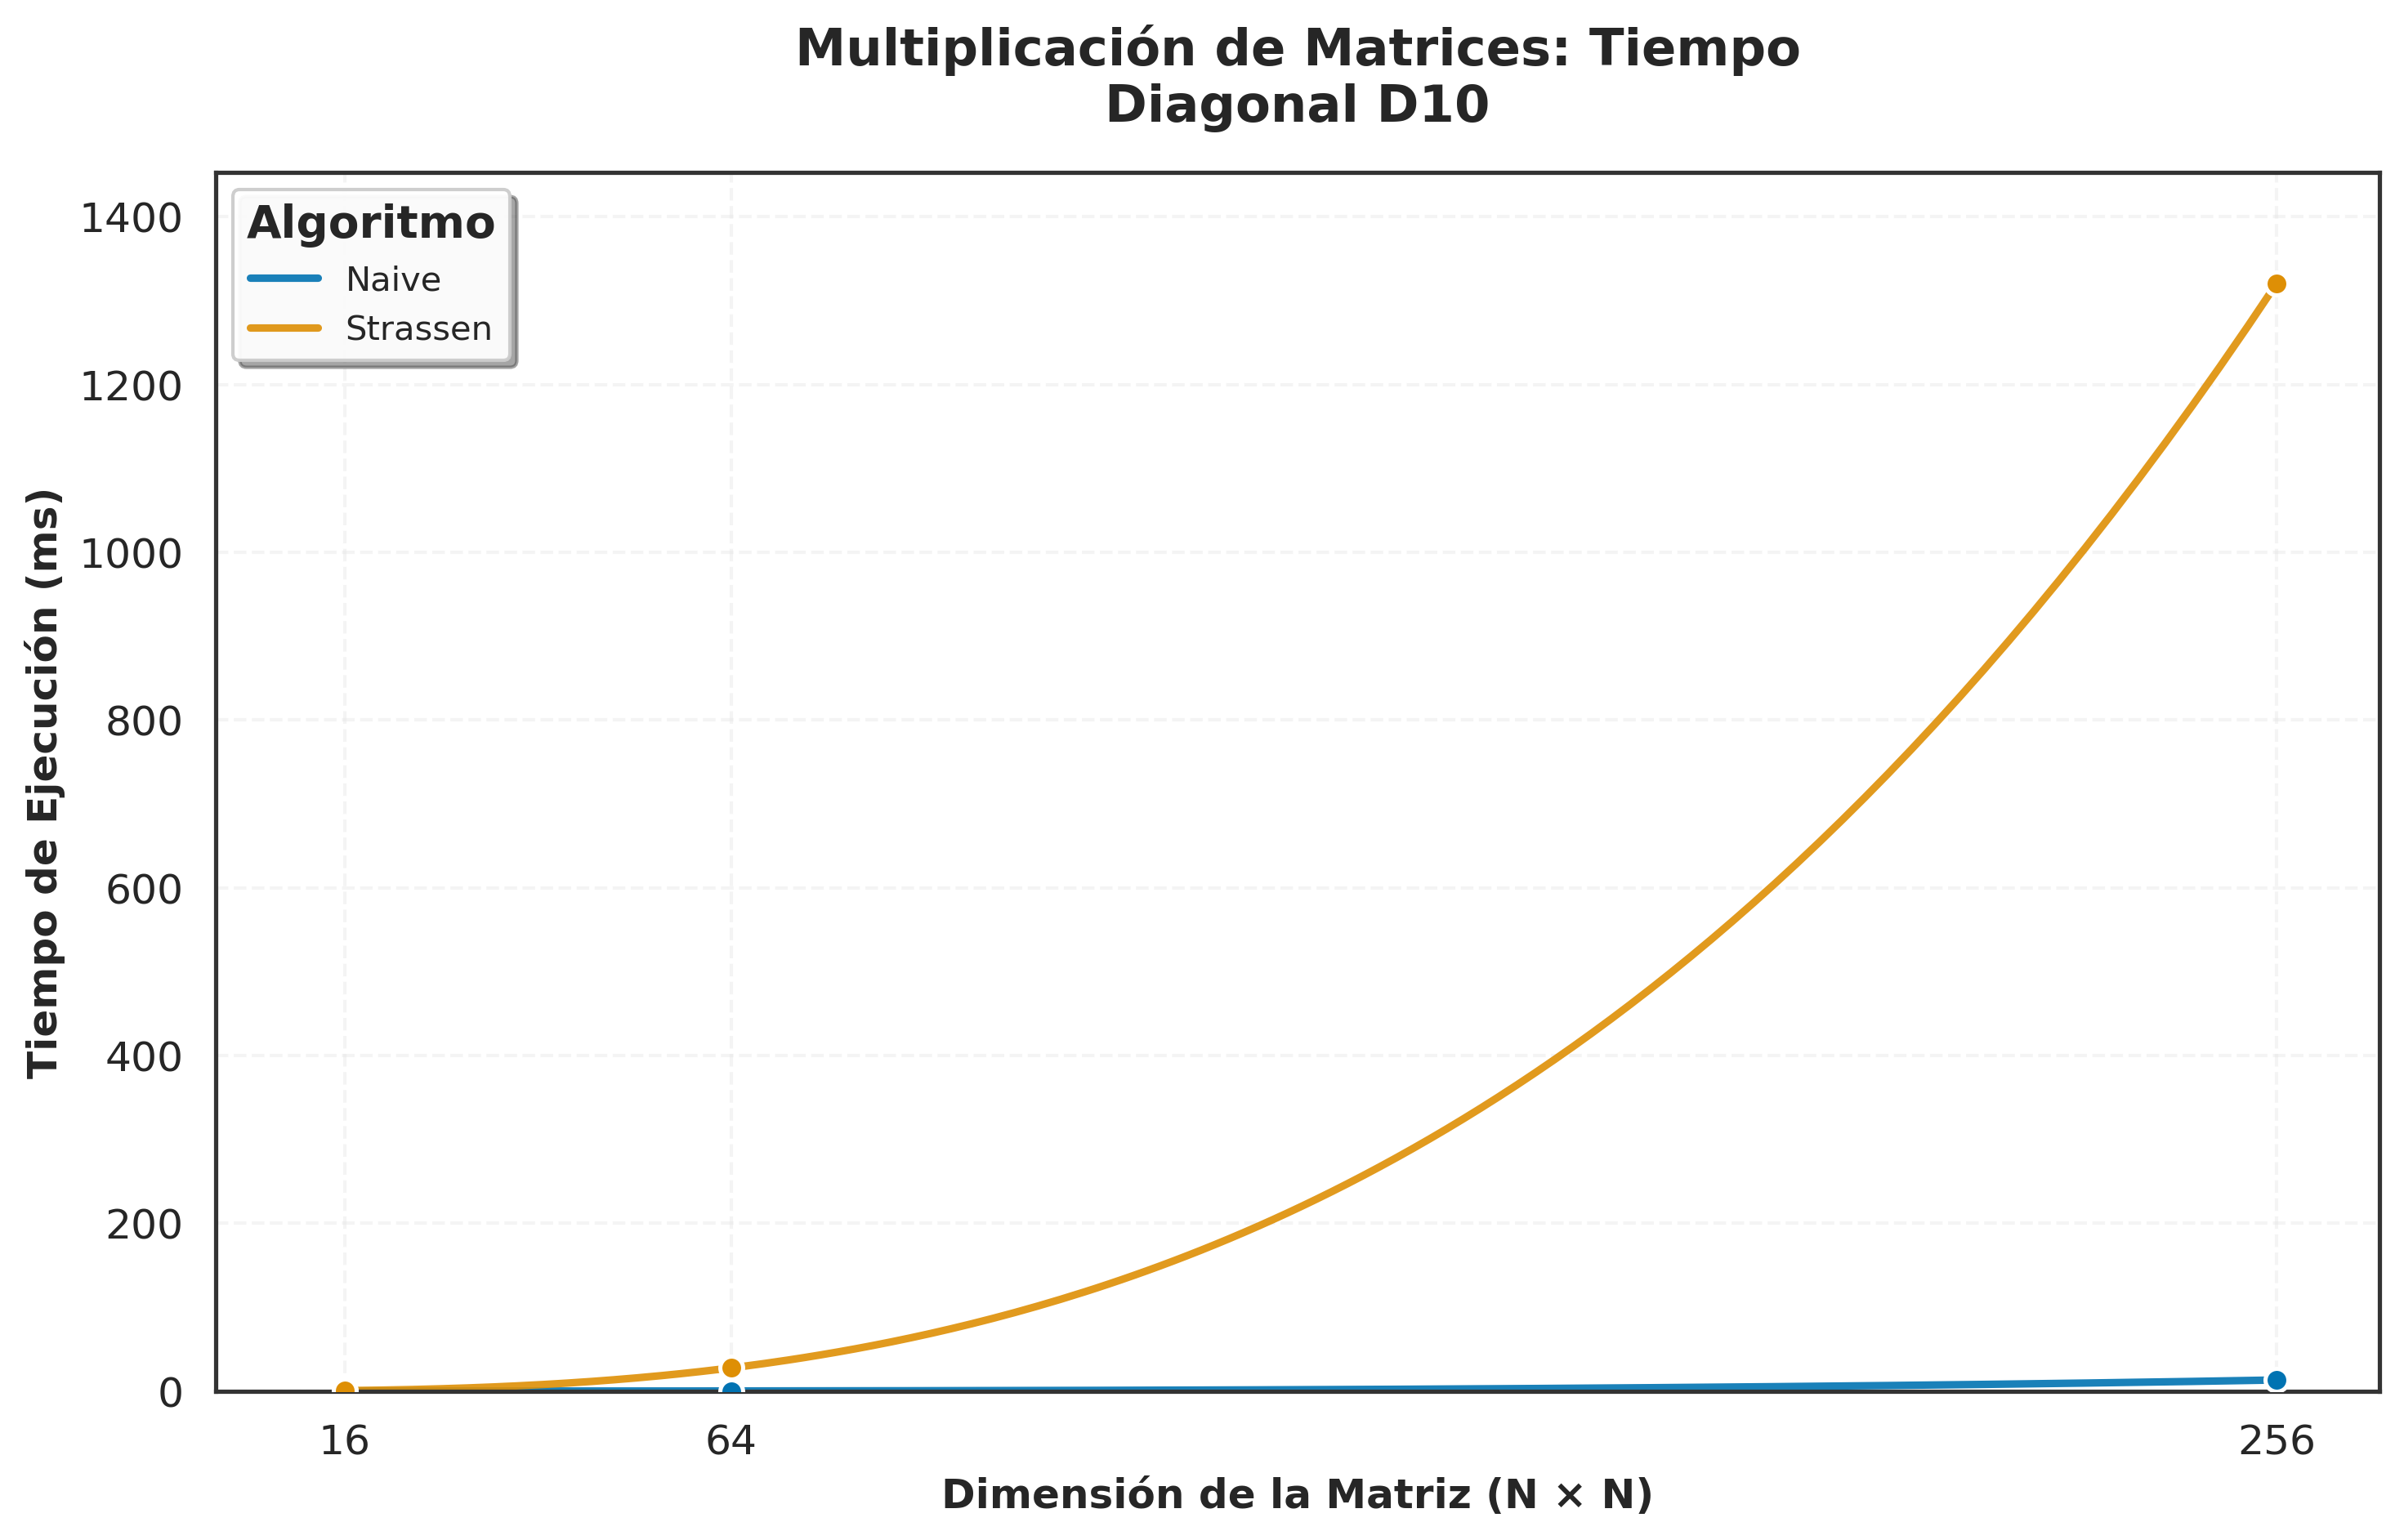
\includegraphics[width=\linewidth]{../code/matrix_multiplication/data/plots/tiempo_diagonal_D10.png}
    \caption{Tiempo, matrices diagonales (D10).}
    \label{fig:mat_tiempo_diag10}
\end{minipage}\\[6pt]
\begin{minipage}[t]{0.31\textwidth}
    \centering
    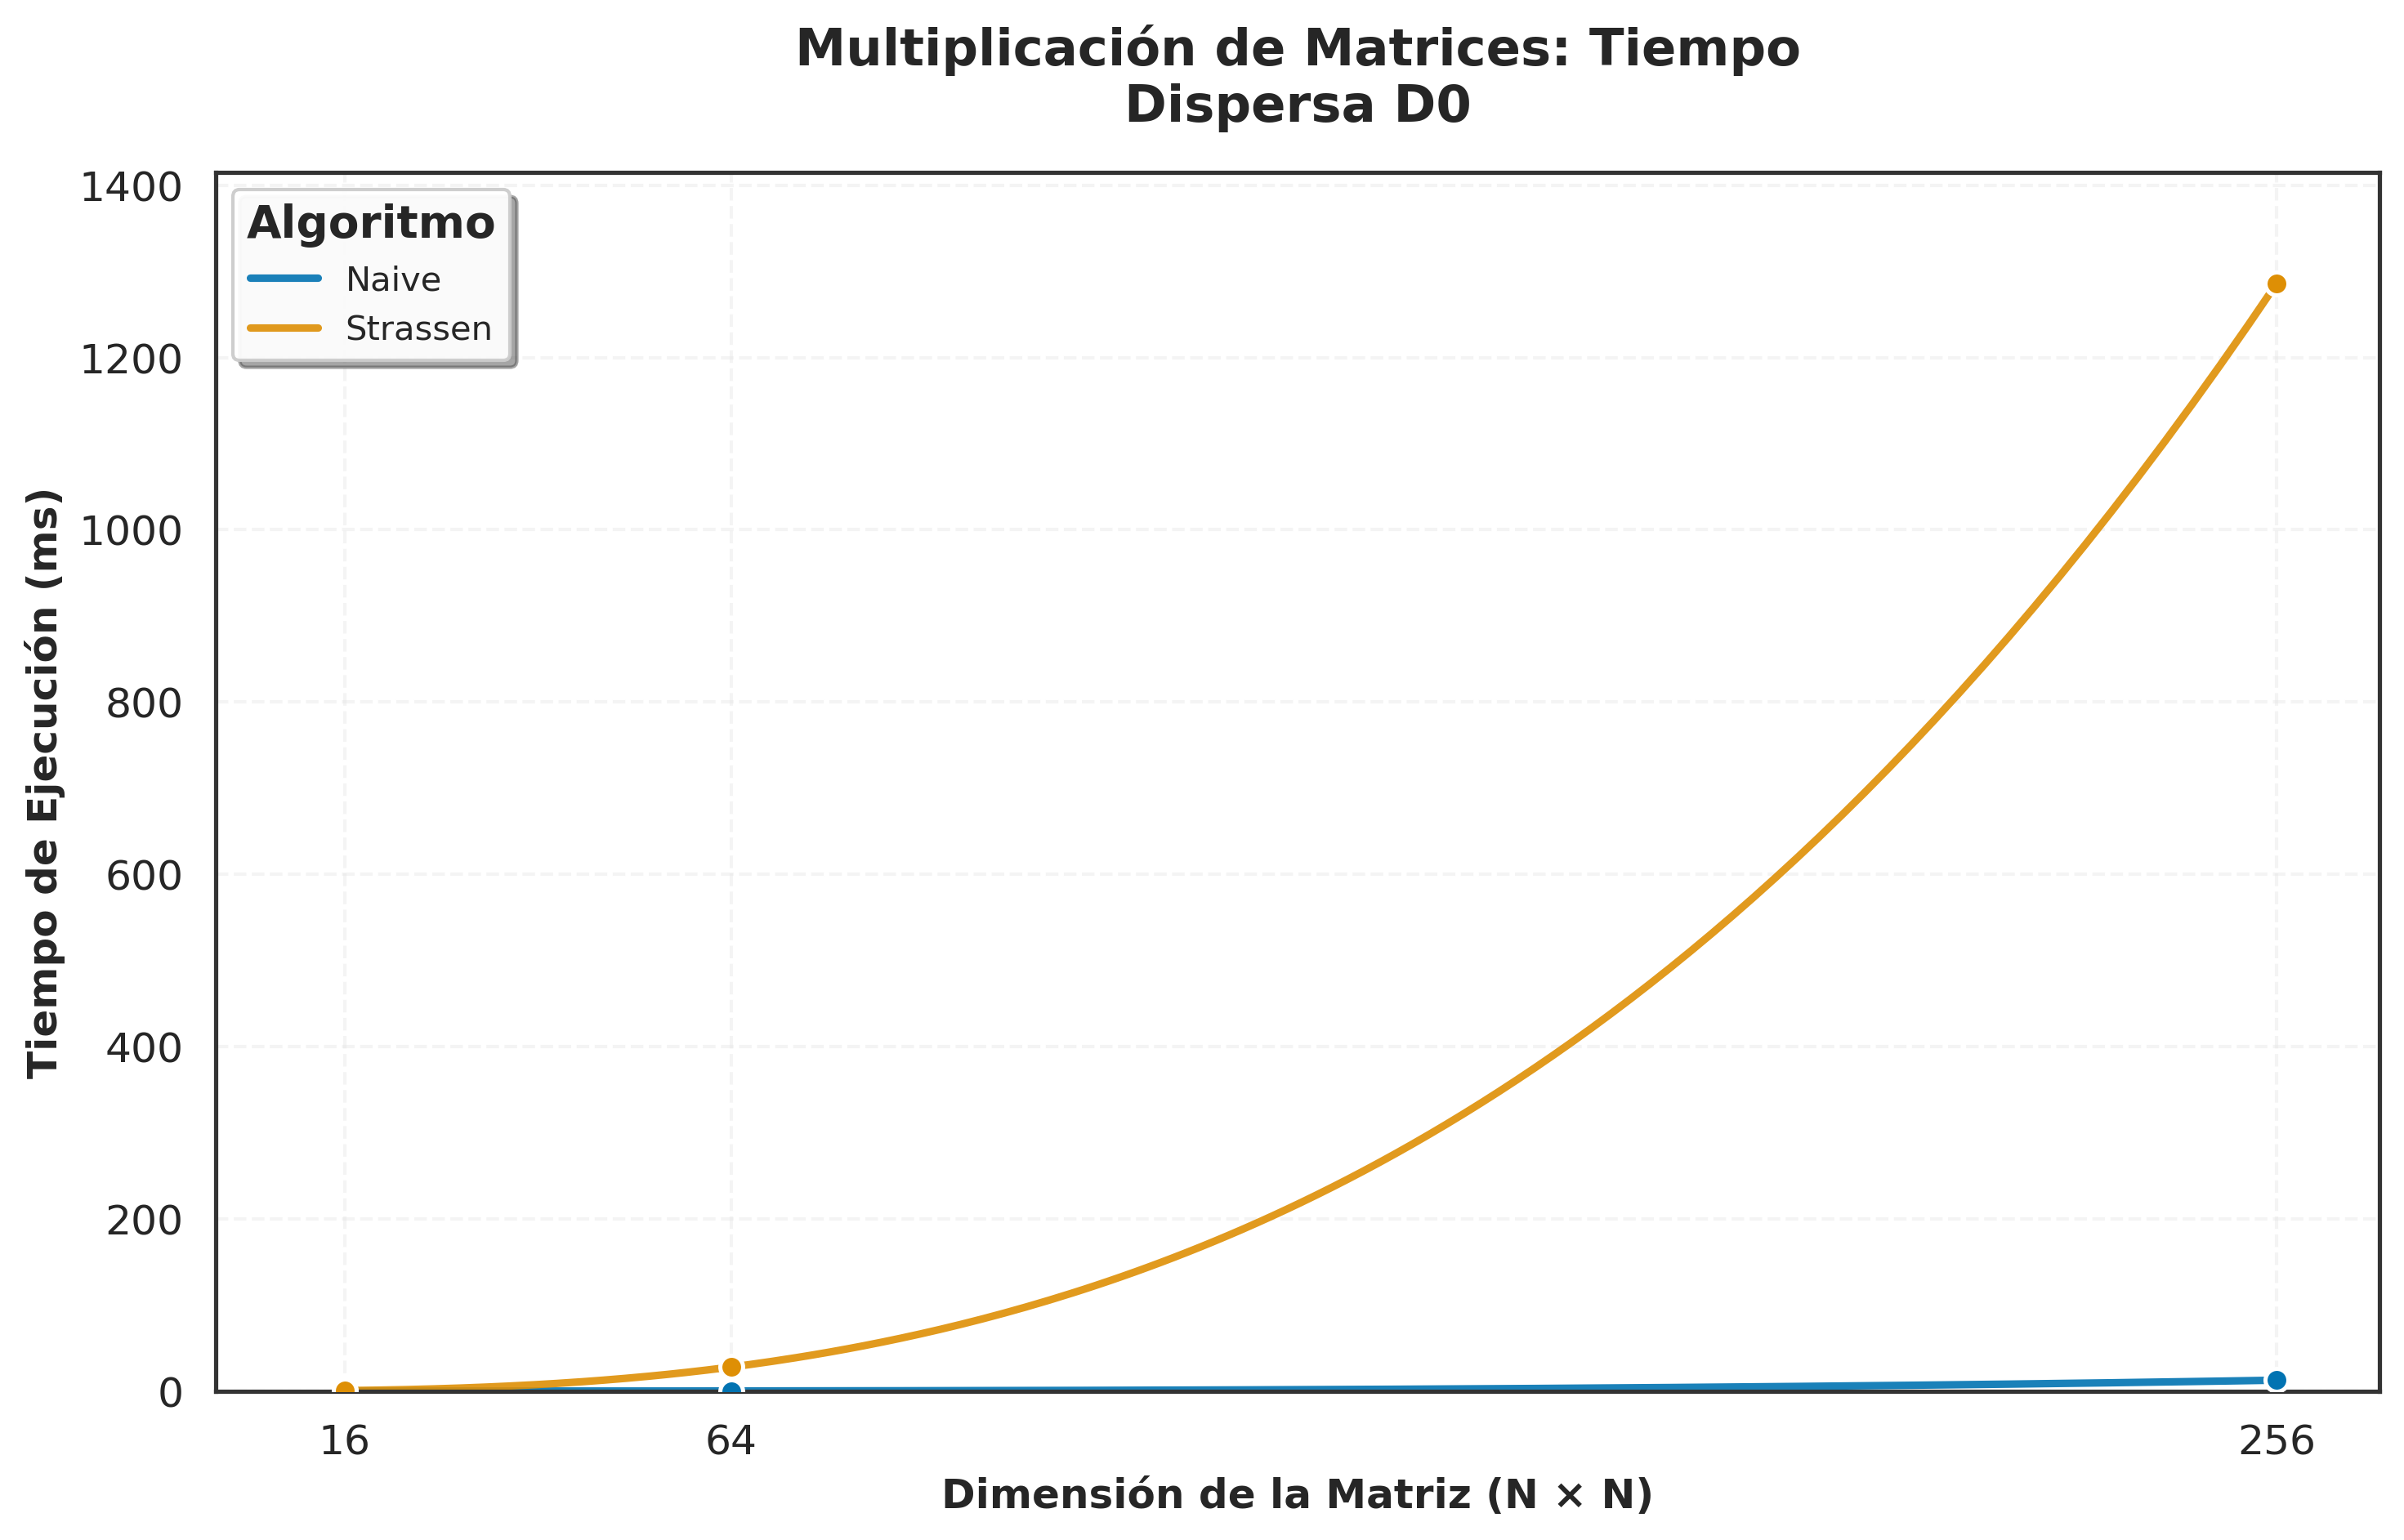
\includegraphics[width=\linewidth]{../code/matrix_multiplication/data/plots/tiempo_dispersa_D0.png}
    \caption{Tiempo, matrices dispersas (D0).}
    \label{fig:mat_tiempo_disp0}
\end{minipage}\hfill
\begin{minipage}[t]{0.31\textwidth}
    \centering
    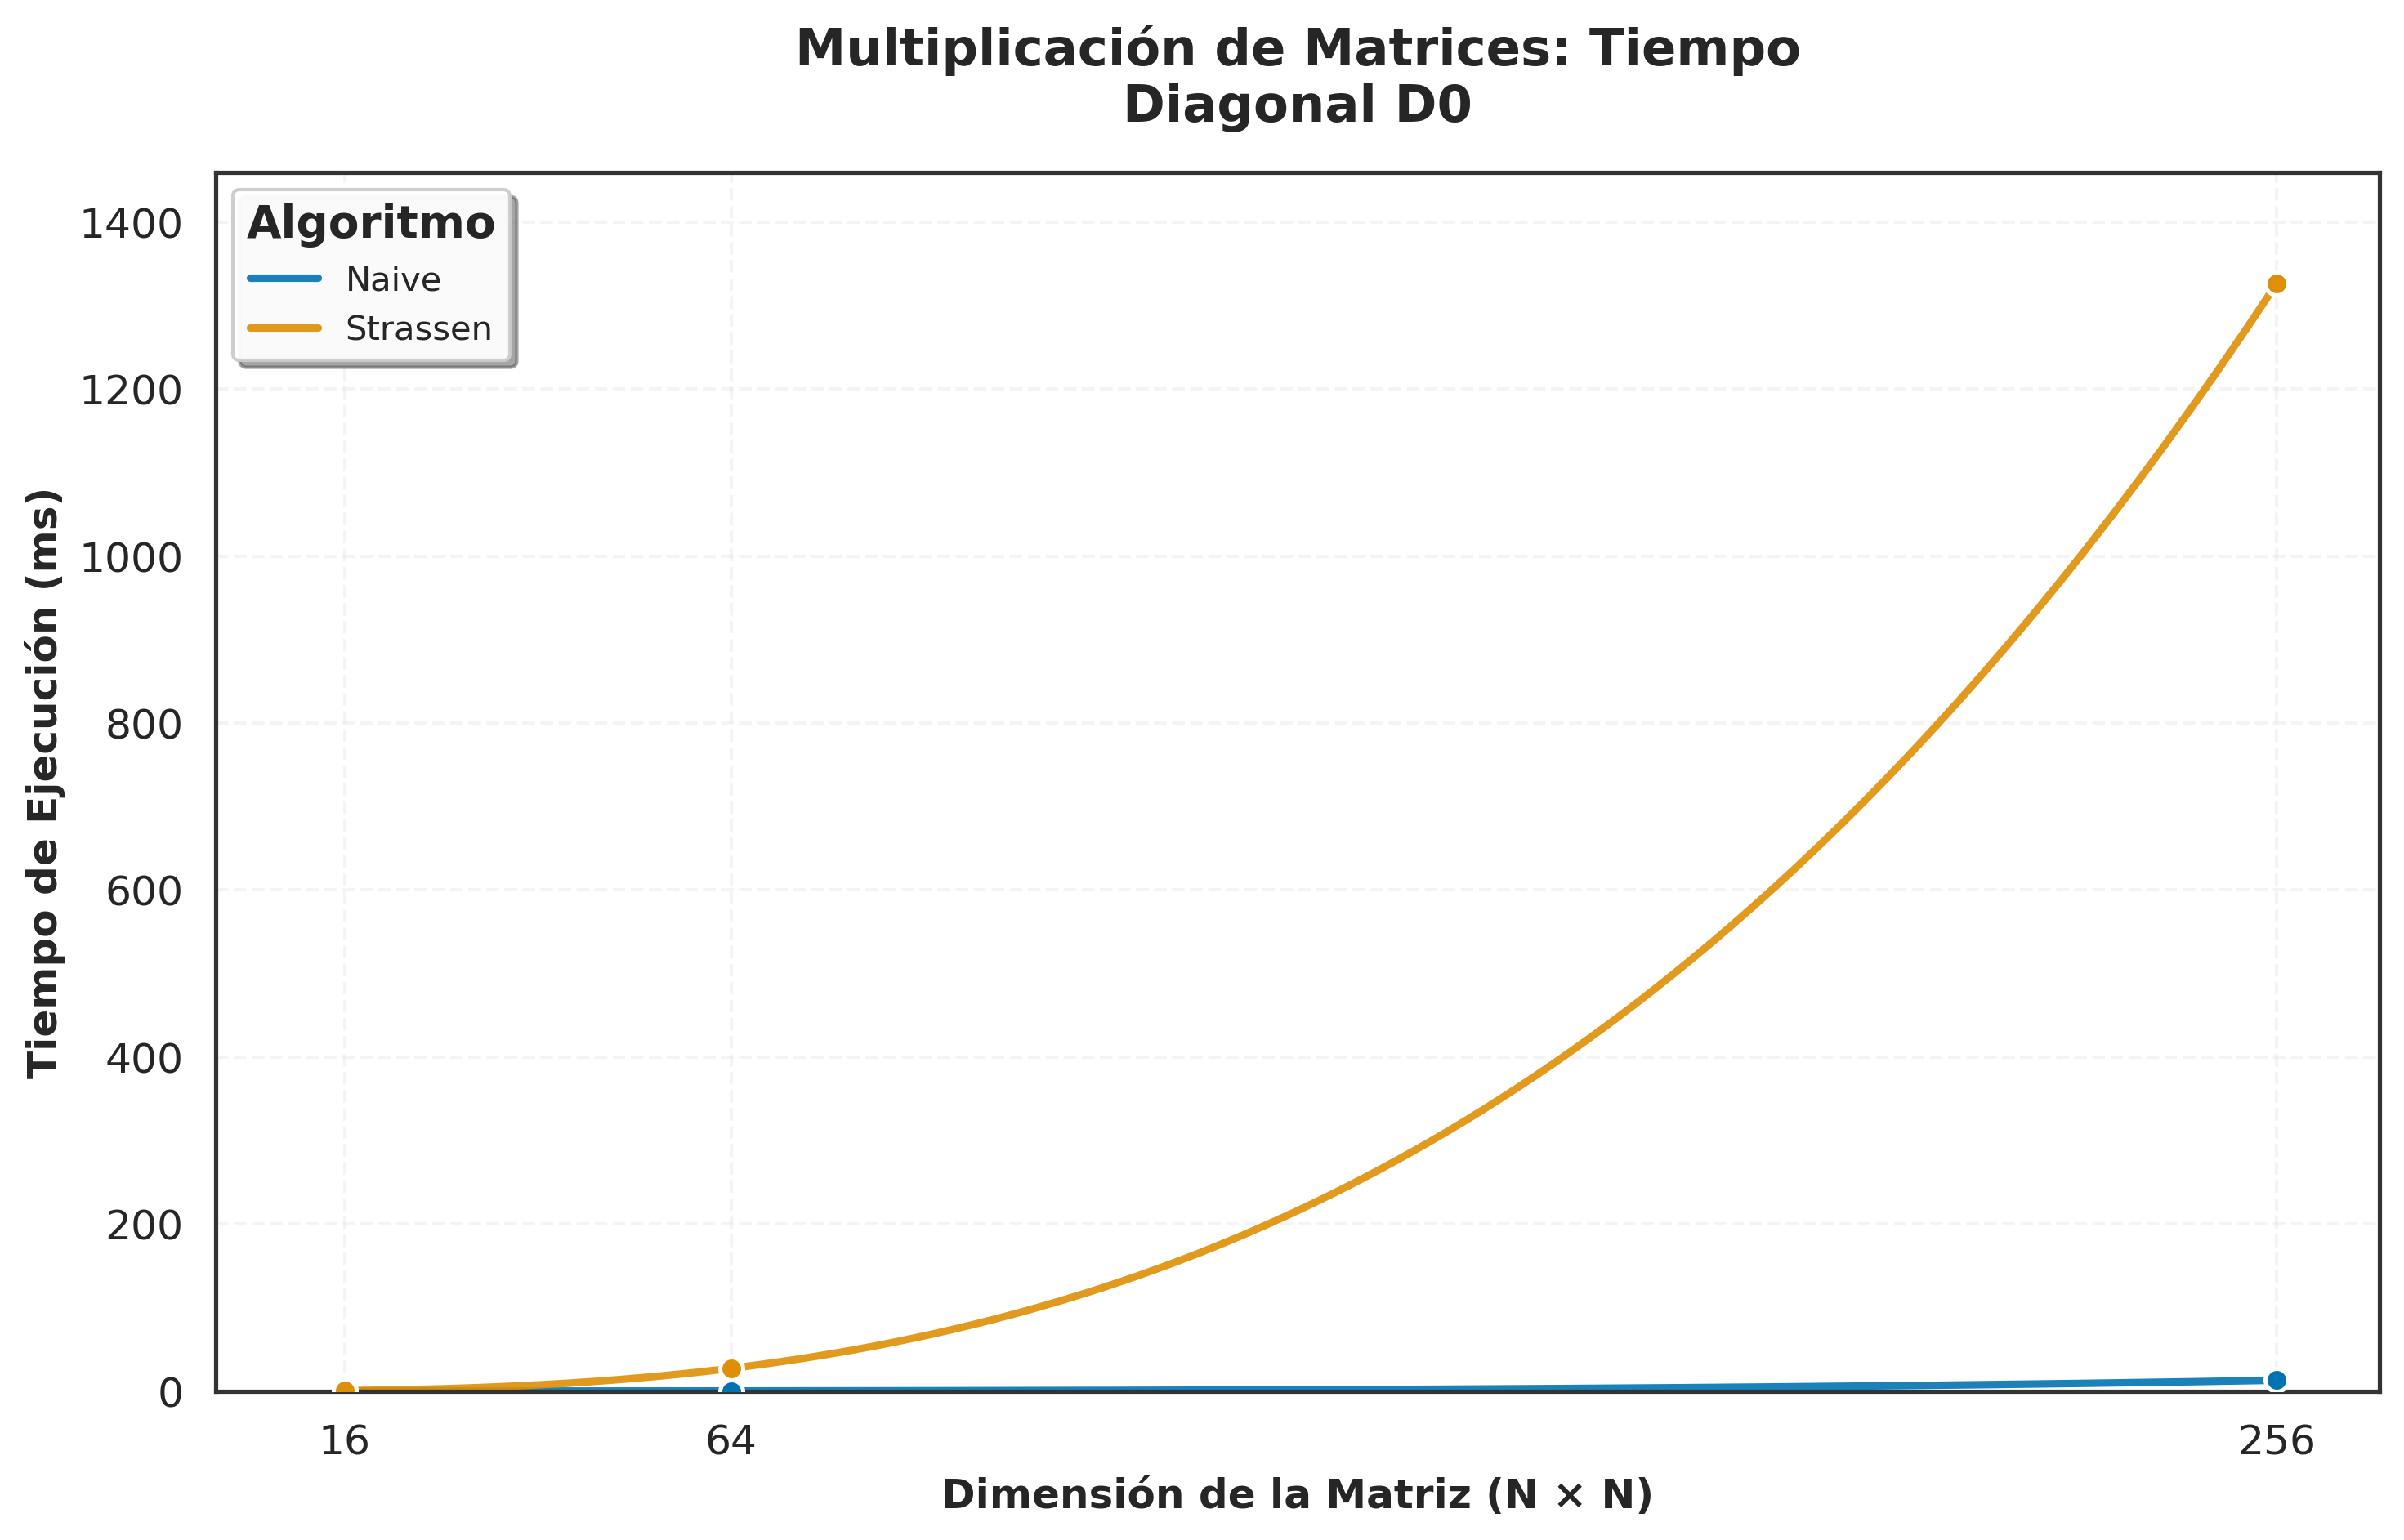
\includegraphics[width=\linewidth]{../code/matrix_multiplication/data/plots/tiempo_diagonal_D0.png}
    \caption{Tiempo, matrices diagonales (D0).}
    \label{fig:mat_tiempo_diag0}
\end{minipage}\hfill
\begin{minipage}[t]{0.31\textwidth}
    \centering
    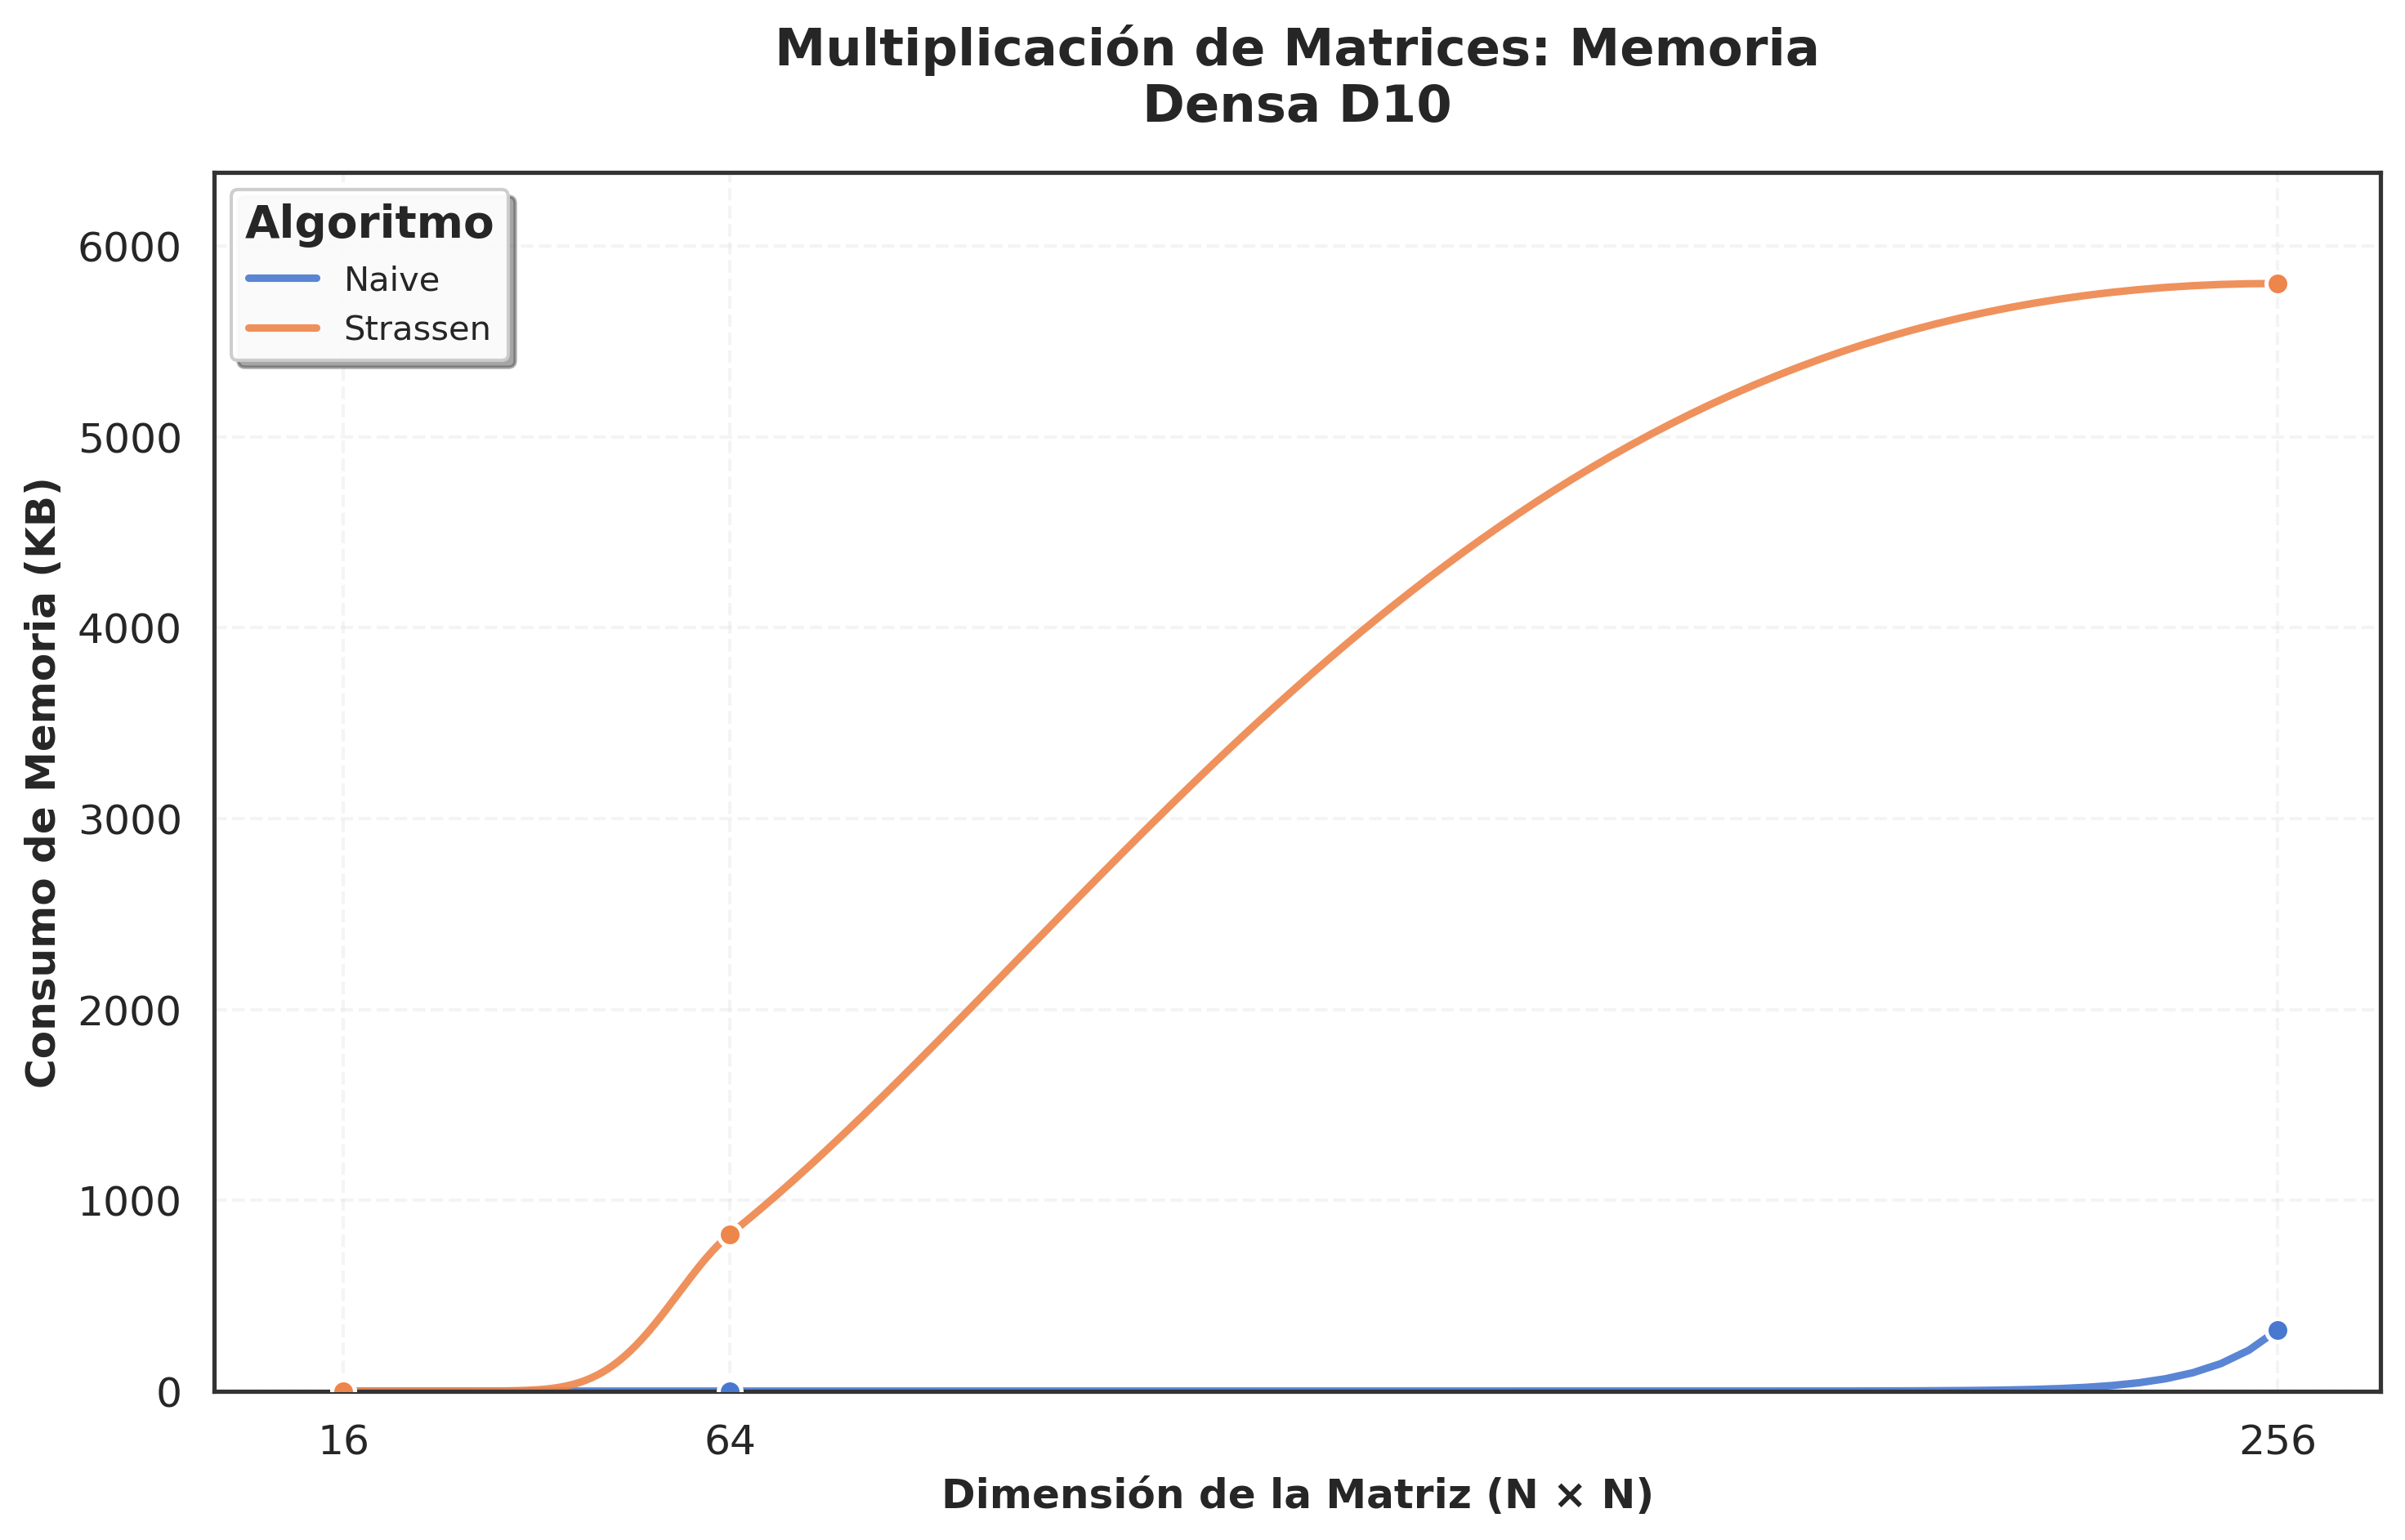
\includegraphics[width=\linewidth]{../code/matrix_multiplication/data/plots/memoria_densa_D10.png}
    \caption{Memoria, matrices densas (D10).}
    \label{fig:mat_mem}
\end{minipage}
\end{figure}


En las figuras 7, 8, 9, 10 y 11 se puede notar que $Strassen$ se demora muchísimo más que $Naive$. Si analizamos la función de recurrencia de $Strassen$ y usamos el teorema maestro se tiene: $T(N) = 7\,T(N/2) + \Theta(N^2)$, donde $a = 7$, $b = 2$, $d = 2$ y como $\log_2 7 \approx 2.81 > 2$ estamos en el caso donde $d < log_ba$ resultando que $T(N) \in \Theta(N^{2,81})$. La teoría nos indica que $Strassen$ debería ser más rápido, sin embargo esto no es así en este caso debido a que las constantes involucradas (debido a las operaciones elementales resultantes de generar matrices temporales en cada nivel de recursión hasta llegar al caso base) son tan grandes que se necesita un $n$ extremadamente grande para que este algoritmo sea más rápido que $Naive$. Es un buen ejemplo de cómo se contrasta la teoría con la práctica. 

En la figura 12 se puede observar que $Strassen$ presenta un consumo muy superior a $Naive$, esto se debe a la memoria auxiliar que se usa debido a las matrices temporales en cada nivel de recursión, mientras que Naive solo requiere la matriz de salida.



\clearpage